%%%%%%%%%%%%%%%%%%%%%%%%%%%%%%%%%%%%%%%%%
% Beamer Presentation
% LaTeX Template
% Version 1.0 (10/11/12)
%
% This template has been downloaded from:
% http://www.LaTeXTemplates.com
%
% License:
% CC BY-NC-SA 3.0 (http://creativecommons.org/licenses/by-nc-sa/3.0/)
%%%%%%%%%%%%%%%%%%%%%%%%%%%%%%%%%%%%%%%%%
%----------------------------------------------------------------------------------------
%	PACKAGES AND THEMES
%----------------------------------------------------------------------------------------

\documentclass{beamer}

\mode<presentation> {

% The Beamer class comes with a number of default slide themes
% which change the colors and layouts of slides. Below this is a list
% of all the themes, uncomment each in turn to see what they look like.

%\usetheme{default}
%\usetheme{AnnArbor}
%\usetheme{Antibes}
%\usetheme{Bergen}
%\usetheme{Berkeley}
%\usetheme{Berlin}
%\usetheme{Boadilla}
%\usetheme{CambridgeUS}
%\usetheme{Copenhagen}
%\usetheme{Darmstadt}
%\usetheme{Dresden}
%\usetheme{Frankfurt}
%\usetheme{Goettingen}
%\usetheme{Hannover}
%\usetheme{Ilmenau}
%\usetheme{JuanLesPins}
%\usetheme{Luebeck}
\usetheme{Madrid}
%\usetheme{Malmoe}
%\usetheme{Marburg}
%\usetheme{Montpellier}
%\usetheme{PaloAlto}
%\usetheme{Pittsburgh}
%\usetheme{Rochester}
%\usetheme{Singapore}
%\usetheme{Szeged}
%\usetheme{Warsaw}

% As well as themes, the Beamer class has a number of color themes
% for any slide theme. Uncomment each of these in turn to see how it
% changes the colors of your current slide theme.

%\usecolortheme{albatross}
%\usecolortheme{beaver}
%\usecolortheme{beetle}
%\usecolortheme{crane}
%\usecolortheme{dolphin}
%\usecolortheme{dove}
%\usecolortheme{fly}
%\usecolortheme{lily}
%\usecolortheme{orchid}
%\usecolortheme{rose}
%\usecolortheme{seagull}
%\usecolortheme{seahorse}
%\usecolortheme{whale}
%\usecolortheme{wolverine}

%\setbeamertemplate{footline} % To remove the footer line in all slides uncomment this line
%\setbeamertemplate{footline}[page number] % To replace the footer line in all slides with a simple slide count uncomment this line

%\setbeamertemplate{navigation symbols}{} % To remove the navigation symbols from the bottom of all slides uncomment this line
}

\usepackage{graphicx} % Allows including images
\usepackage{booktabs} % Allows the use of \toprule, \midrule and \bottomrule in tables


%%%% MY imported items %%%
\setbeamercovered{invisibel}
%\setbeamercovered{dynamic}
%%%%%%%%%%%%%%%%%%%%%%%%%

%----------------------------------------------------------------------------------------
%	TITLE PAGE
%----------------------------------------------------------------------------------------

\title[Interview Presentation]{Interview Presentation} % The short title appears at the bottom of every slide, the full title is only on the title page

\author{Yayang Tian} % Your name
\institute[UPenn] % Your institution as it will appear on the bottom of every slide, may be shorthand to save space
{
University of Pennsylvania \\ % Your institution for the title page
\medskip
\textit{yayangtian@gmail.com} % Your email address
}
\date{\today} % Date, can be changed to a custom date

\begin{document}

\begin{frame}
\titlepage % Print the title page as the first slide
\end{frame}





\large

%------------------------------- Intro -----------------

\section{Education}

\begin{frame}
\frametitle{Education}
\textbf{University of Pennlsyvania}
\begin{itemize}
\item M.S.E. in Computer and Information Science, Big Data
\end{itemize}

\textbf{Shanghai Jiao Tong University}
\begin{itemize}
\item B.E. in Information Science, Honor Class
\end{itemize}

\textbf{Shenzhen Middle School}
\begin{itemize}
\item Physics, Honor Class, CPO 1st Prize
\end{itemize}

\end{frame}


\section{Experience}

\textbf{Software Engineer - Walmart Labs, Sunnyvale}
\begin{itemize}
\item Online shopping personalization. 
\item Advertisement matching.
\end{itemize}

\textbf{Software Engineer - Microsoft, Boston}
\begin{itemize}
\item AWS Map Reduce Jobs.
\item Windows Phone Apps. 
\end{itemize}

\begin{frame}
\frametitle{Experience}
\textbf{Research Assitant - NLP, University of Pennlsyvania}
\begin{itemize}
\item Emotion classification with unsupervised learning.
\item Implicit expressions of emotion in text. Python.
\end{itemize}

\textbf{Software Developer - CS Dept, University of Pennlsyvania}
\begin{itemize}
\item Automatic methods to measure quality in text.
\item Crowdsourcing websites for data mining. Php/MySQL.
\end{itemize}

\end{frame}



\section{Projects}


\begin{frame}

\frametitle{Projects Overview}

\textbf{Distributed Systems}
\begin{itemize}
\item Distributed Web Search Engine: MiniGoogle
\item DHT-based Search Engine: PennSearch 
\item Distributed Caching and Web Services
\item Web Crawler with Multithreaded Server 
\end{itemize}


\textbf{Data Mining}
\begin{itemize}
\item Amazon Reviews Data Mining
\item Tweets Emotion Prediction
\item New York Times Summarization
\item Wall Street Journal Crowdsouring Website
\end{itemize}

\textbf{Others}
\begin{itemize}
\item Mobile Applications
\item Database Website on GAE
\end{itemize}

\end{frame}

%------------------------------- MiniGoogle -----------------

\section{Projects}


\subsection{Distributed Web Search Engine - MiniGoogle}

\begin{frame}

\frametitle{MiniGoogle}

\textbf{Techniques}
\begin{itemize} \item Java, Hadoop, MapReduce, AWS, FreePastry, Berkeley DB. \end{itemize}
\textbf{Components}
\begin{itemize} \item Crawler, indexer, PageRank, web UI. \end{itemize}
\textbf{Contribution}
\begin{itemize}
\item MapReduce: TF-IDF information retrieval for indexing;
\item Ranking/Search Relevance: scoring, weighting, ranking; presented new ranking algorithm including 10 features;
\item Website: designed and implemented the website with Twitter Bootstrap and HTML/CSS;
\item Web Services: REST APIs, recommendation engine integration.
\end{itemize}
\end{frame}


\begin{frame}
\frametitle{MiniGoogle}
\begin{figure}
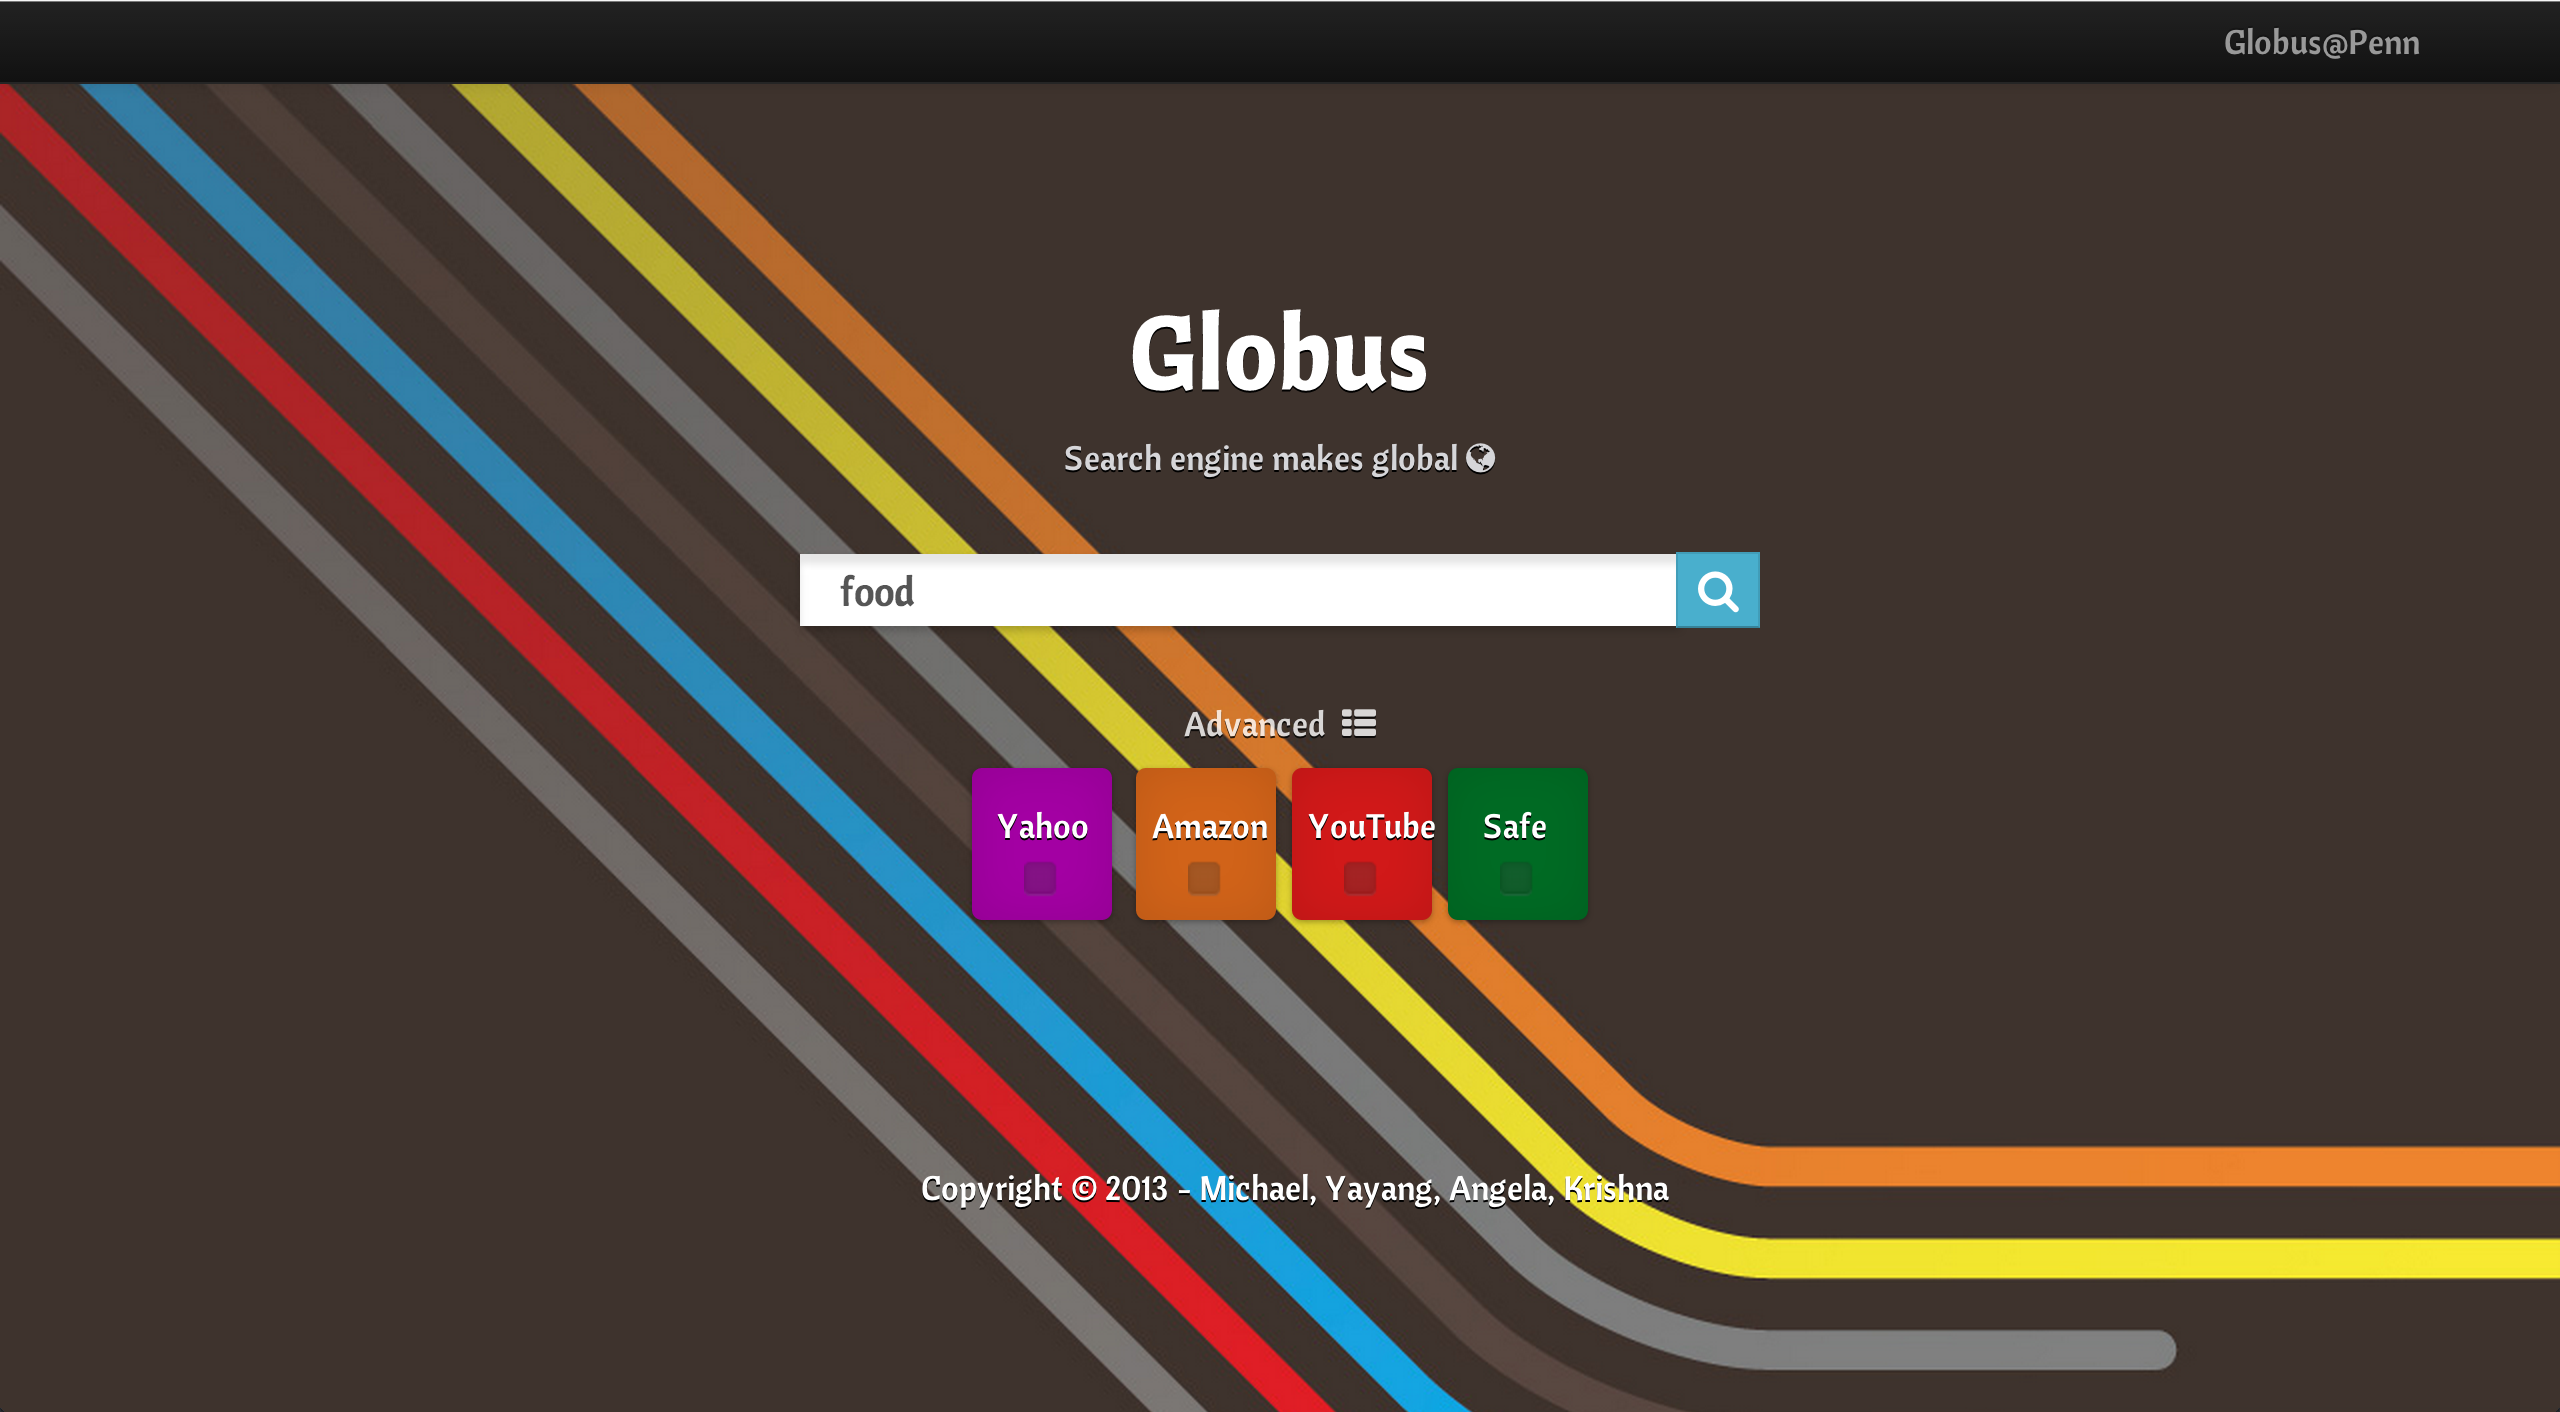
\includegraphics[width=1\linewidth]{pic/search1.png}
\end{figure}
\end{frame}
\begin{frame}
\frametitle{MiniGoogle}
\begin{figure}
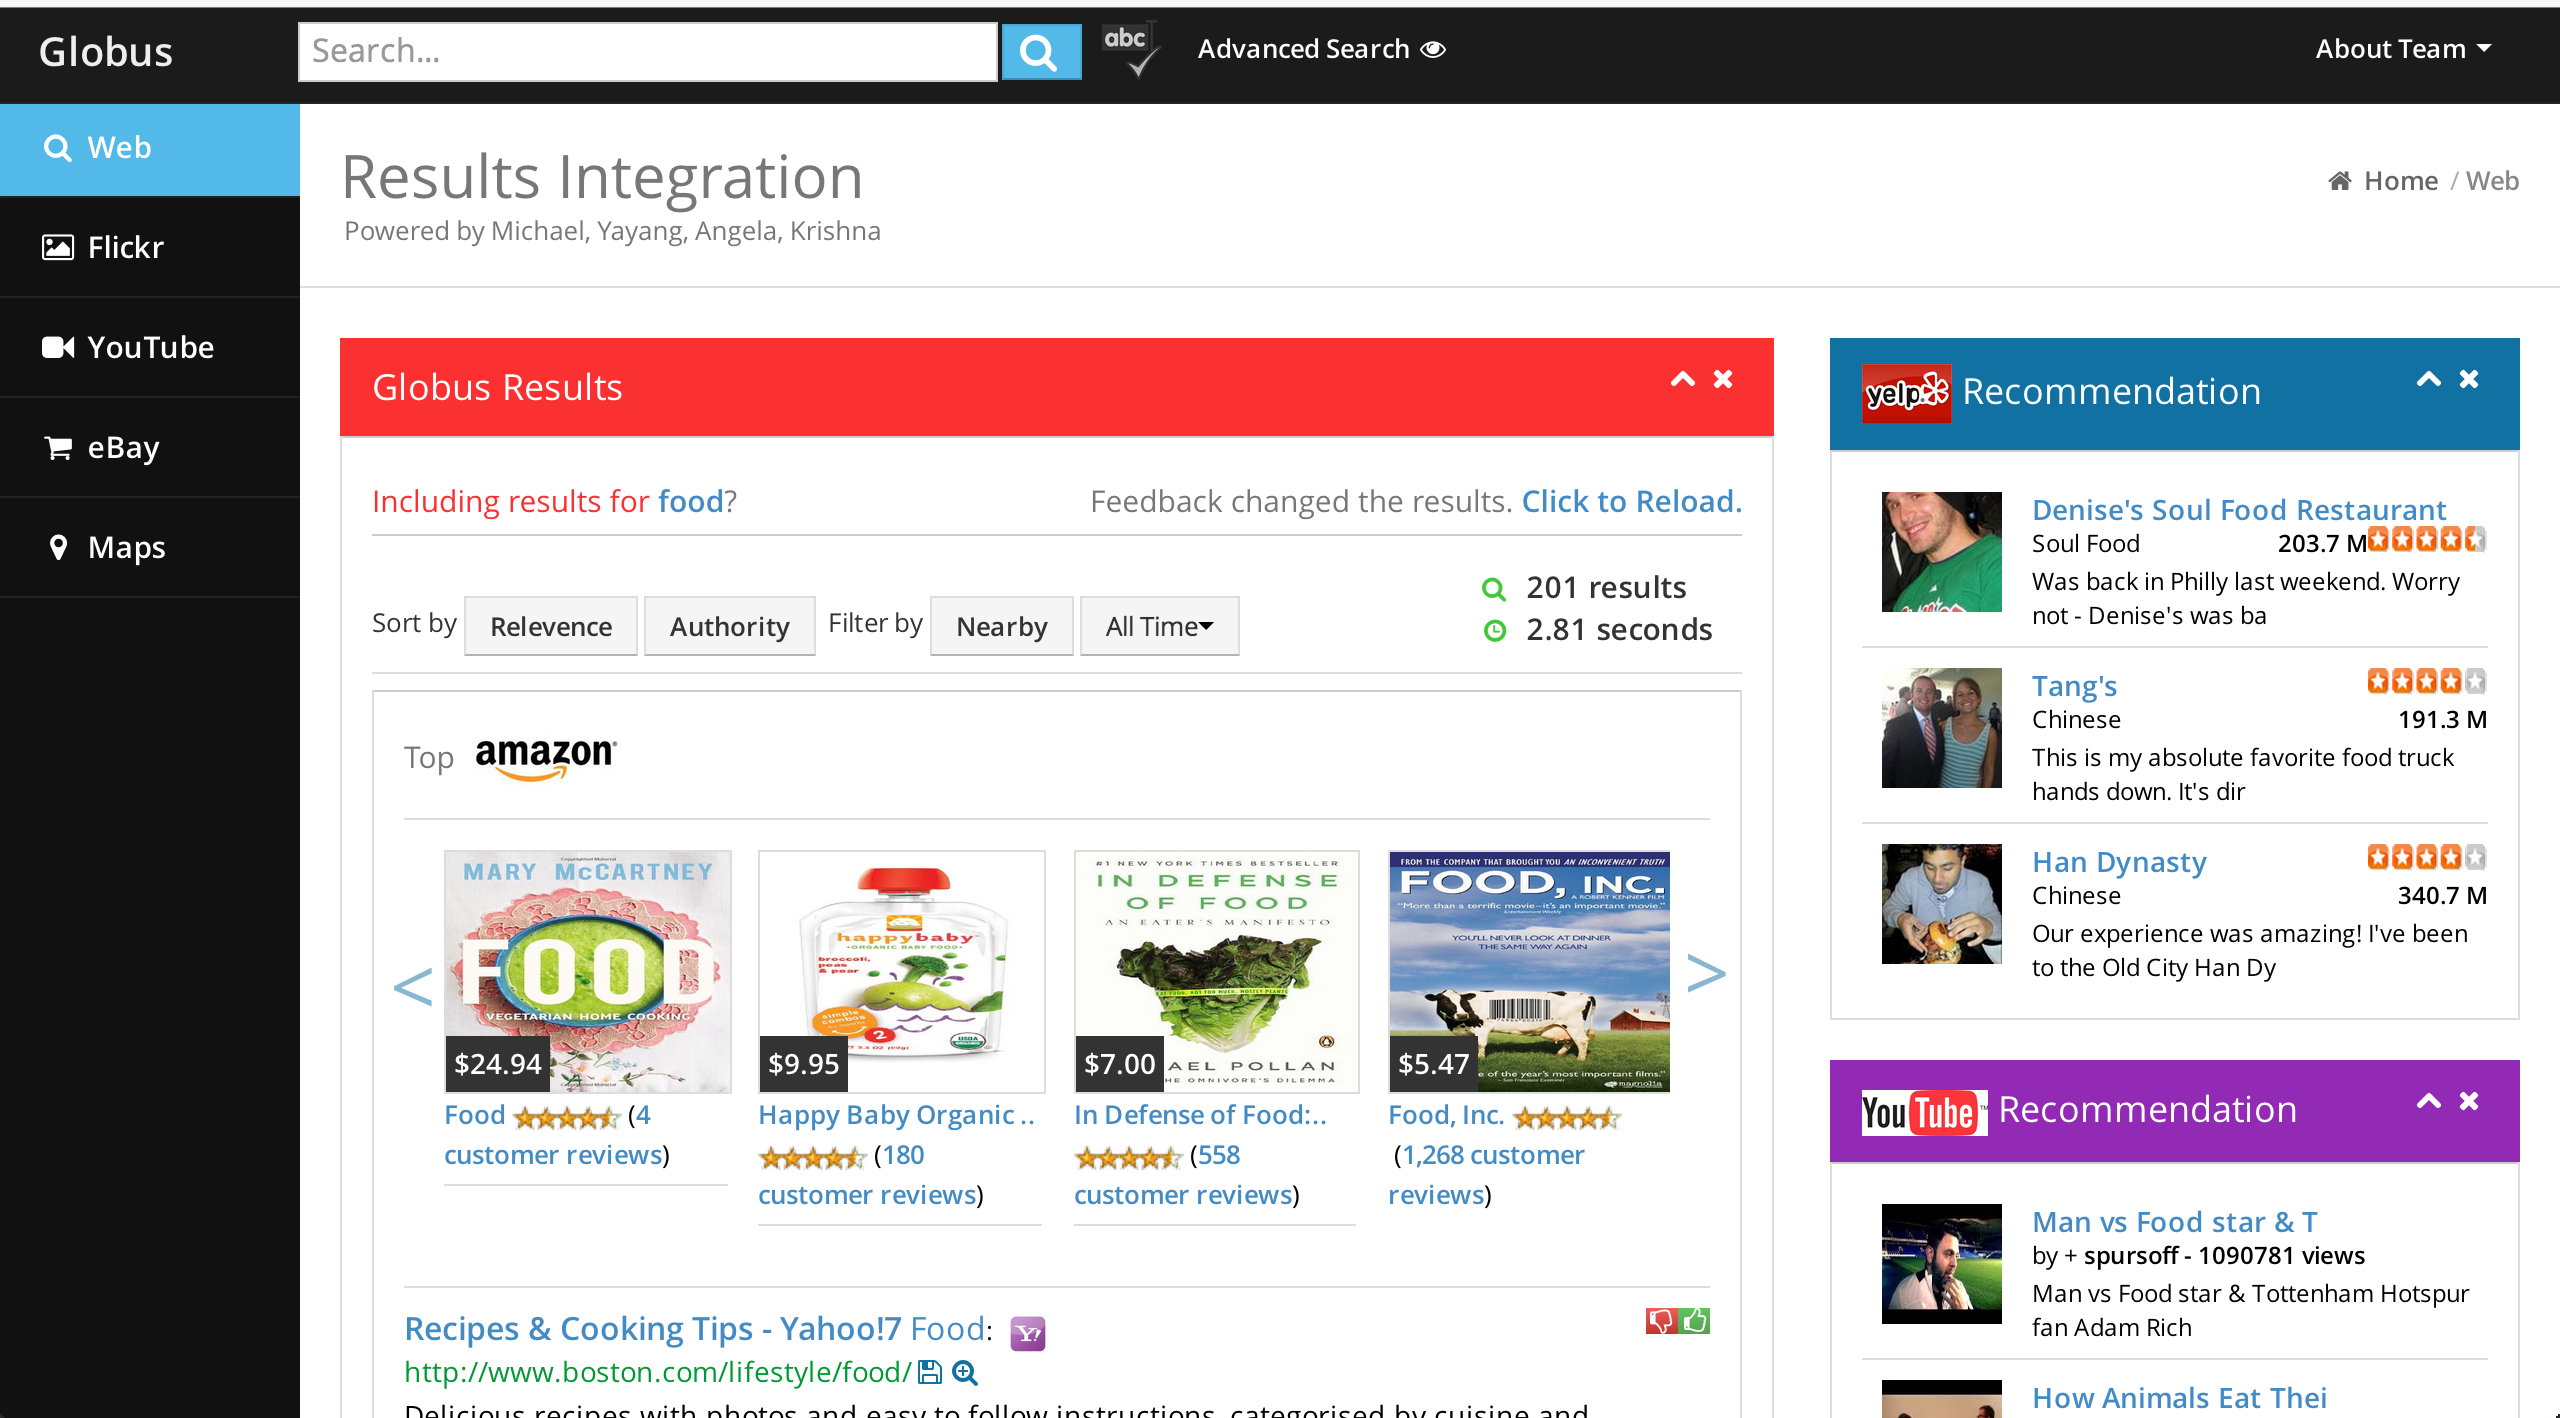
\includegraphics[width=1\linewidth]{pic/search2.png}
\end{figure}
\end{frame}
\begin{frame}
\frametitle{MiniGoogle}
\begin{figure}
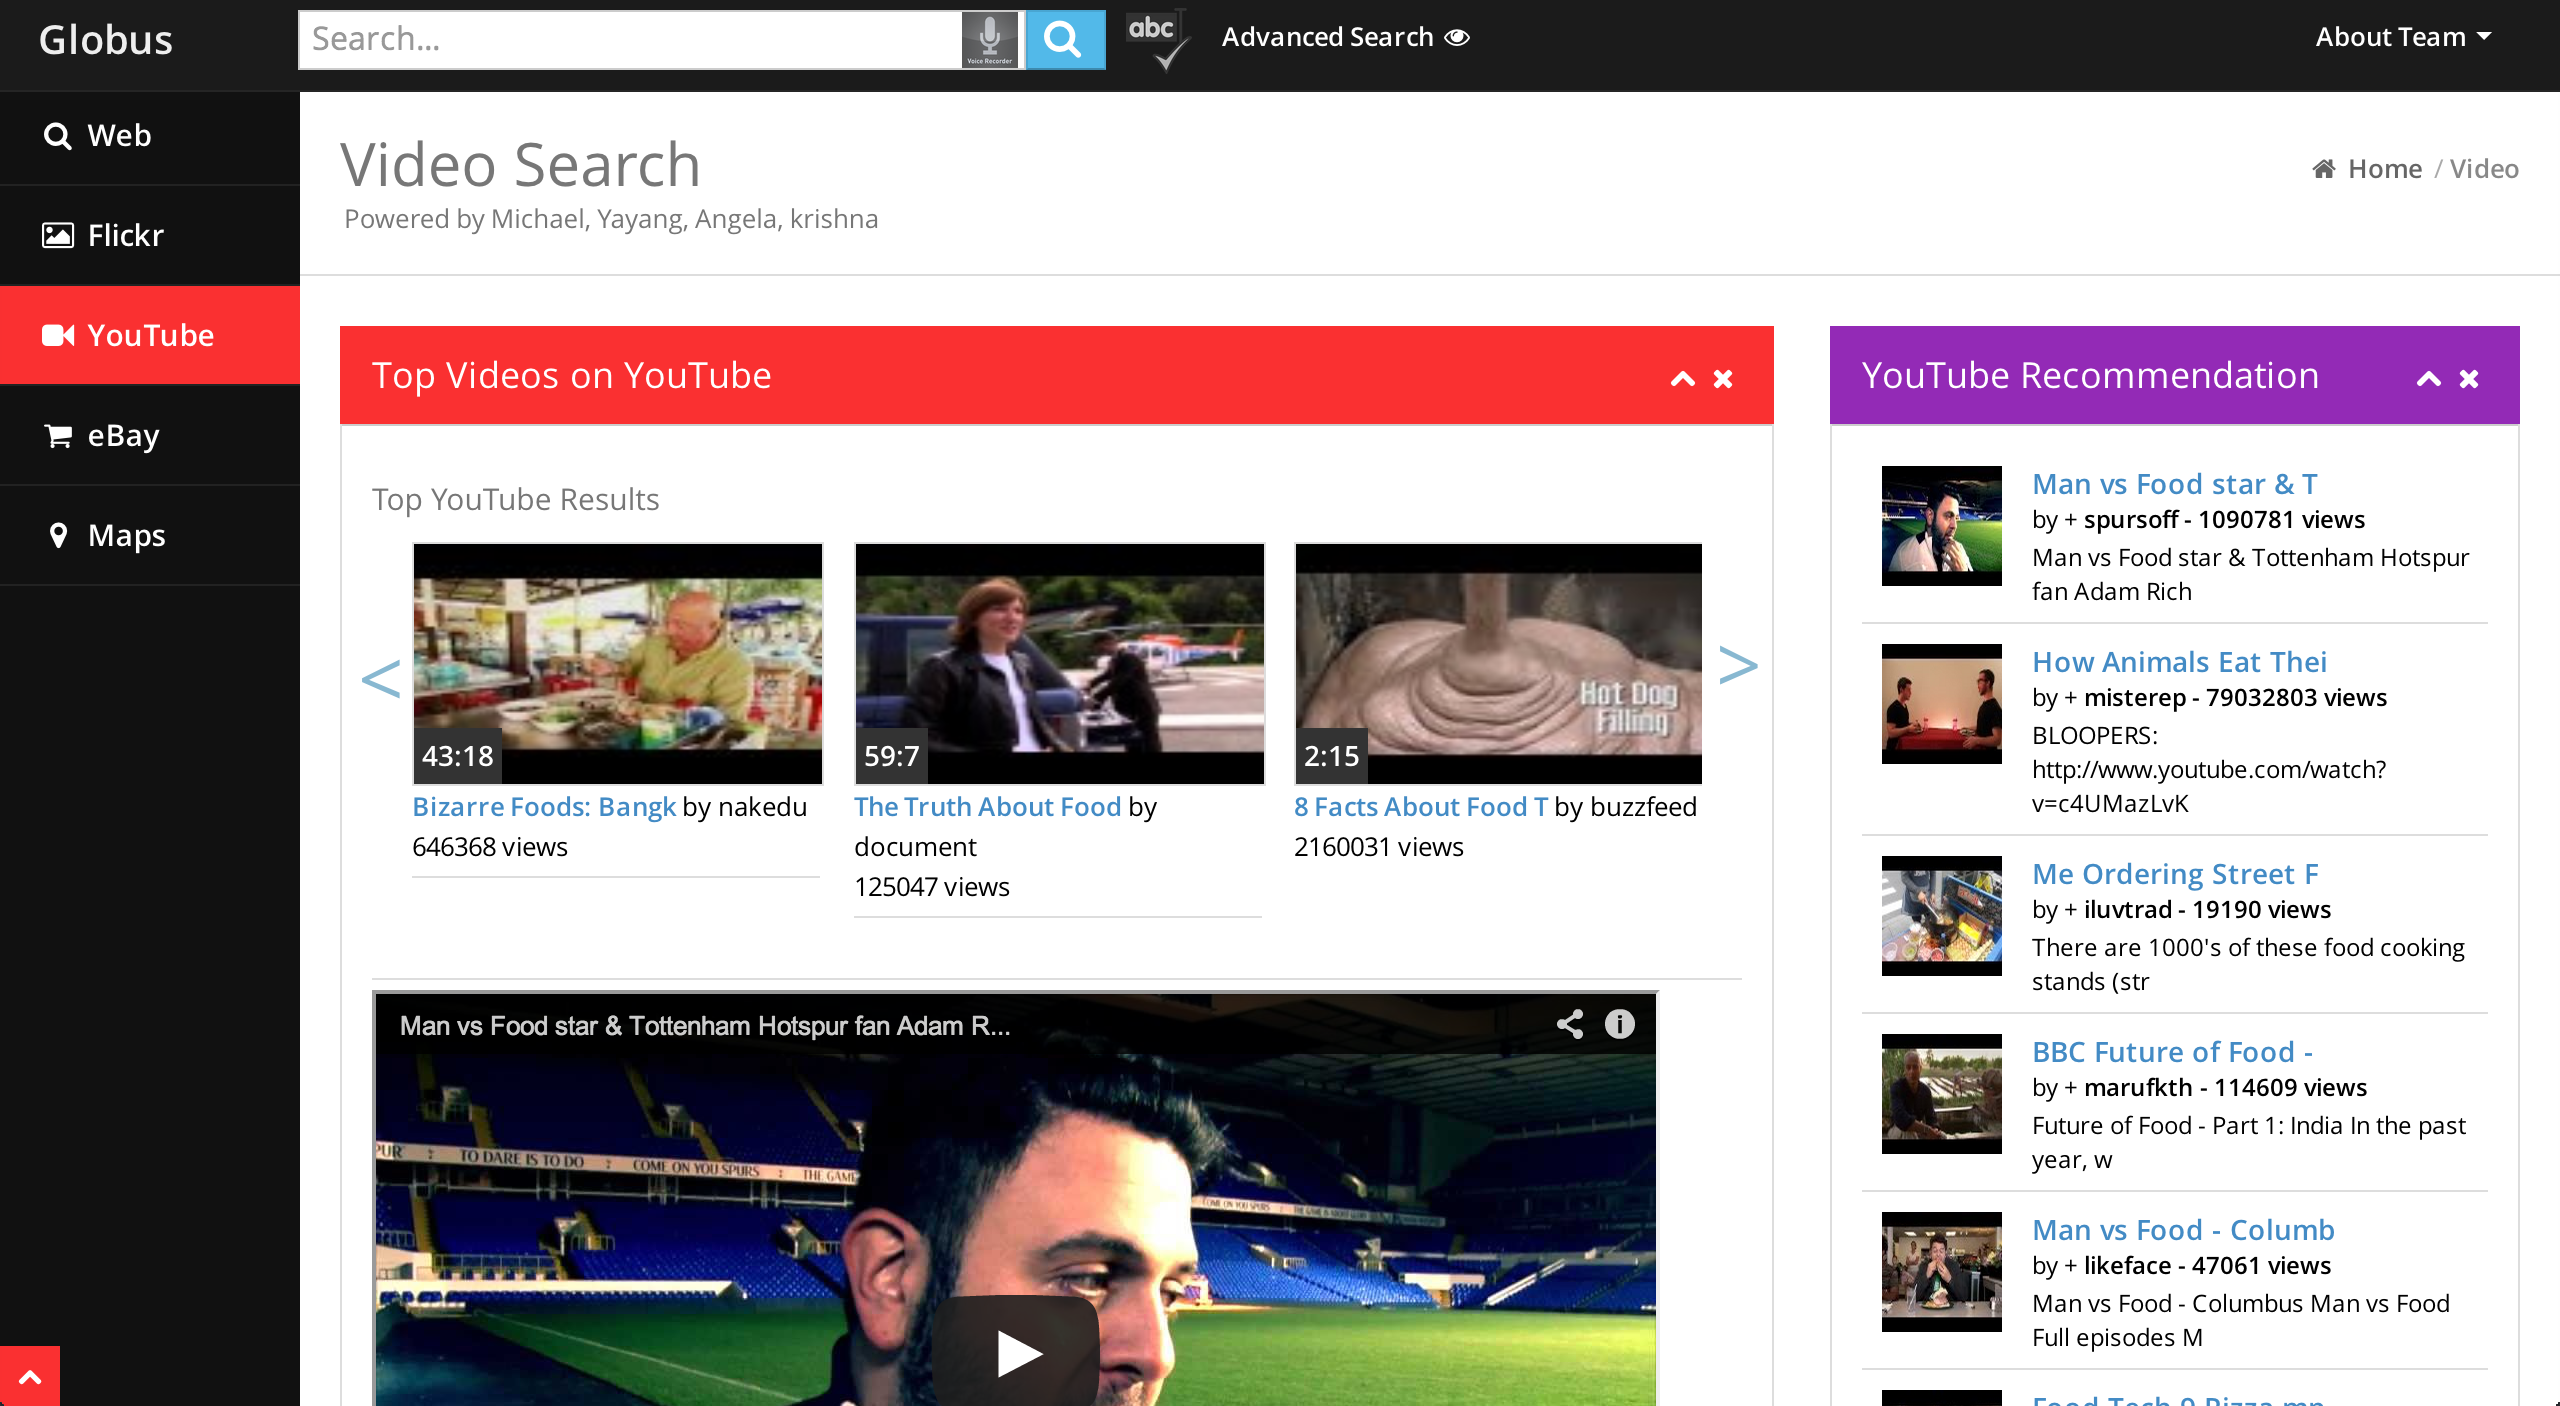
\includegraphics[width=1\linewidth]{pic/search3.png}
\end{figure}
\end{frame}
\begin{frame}
\frametitle{MiniGoogle}
\begin{figure}
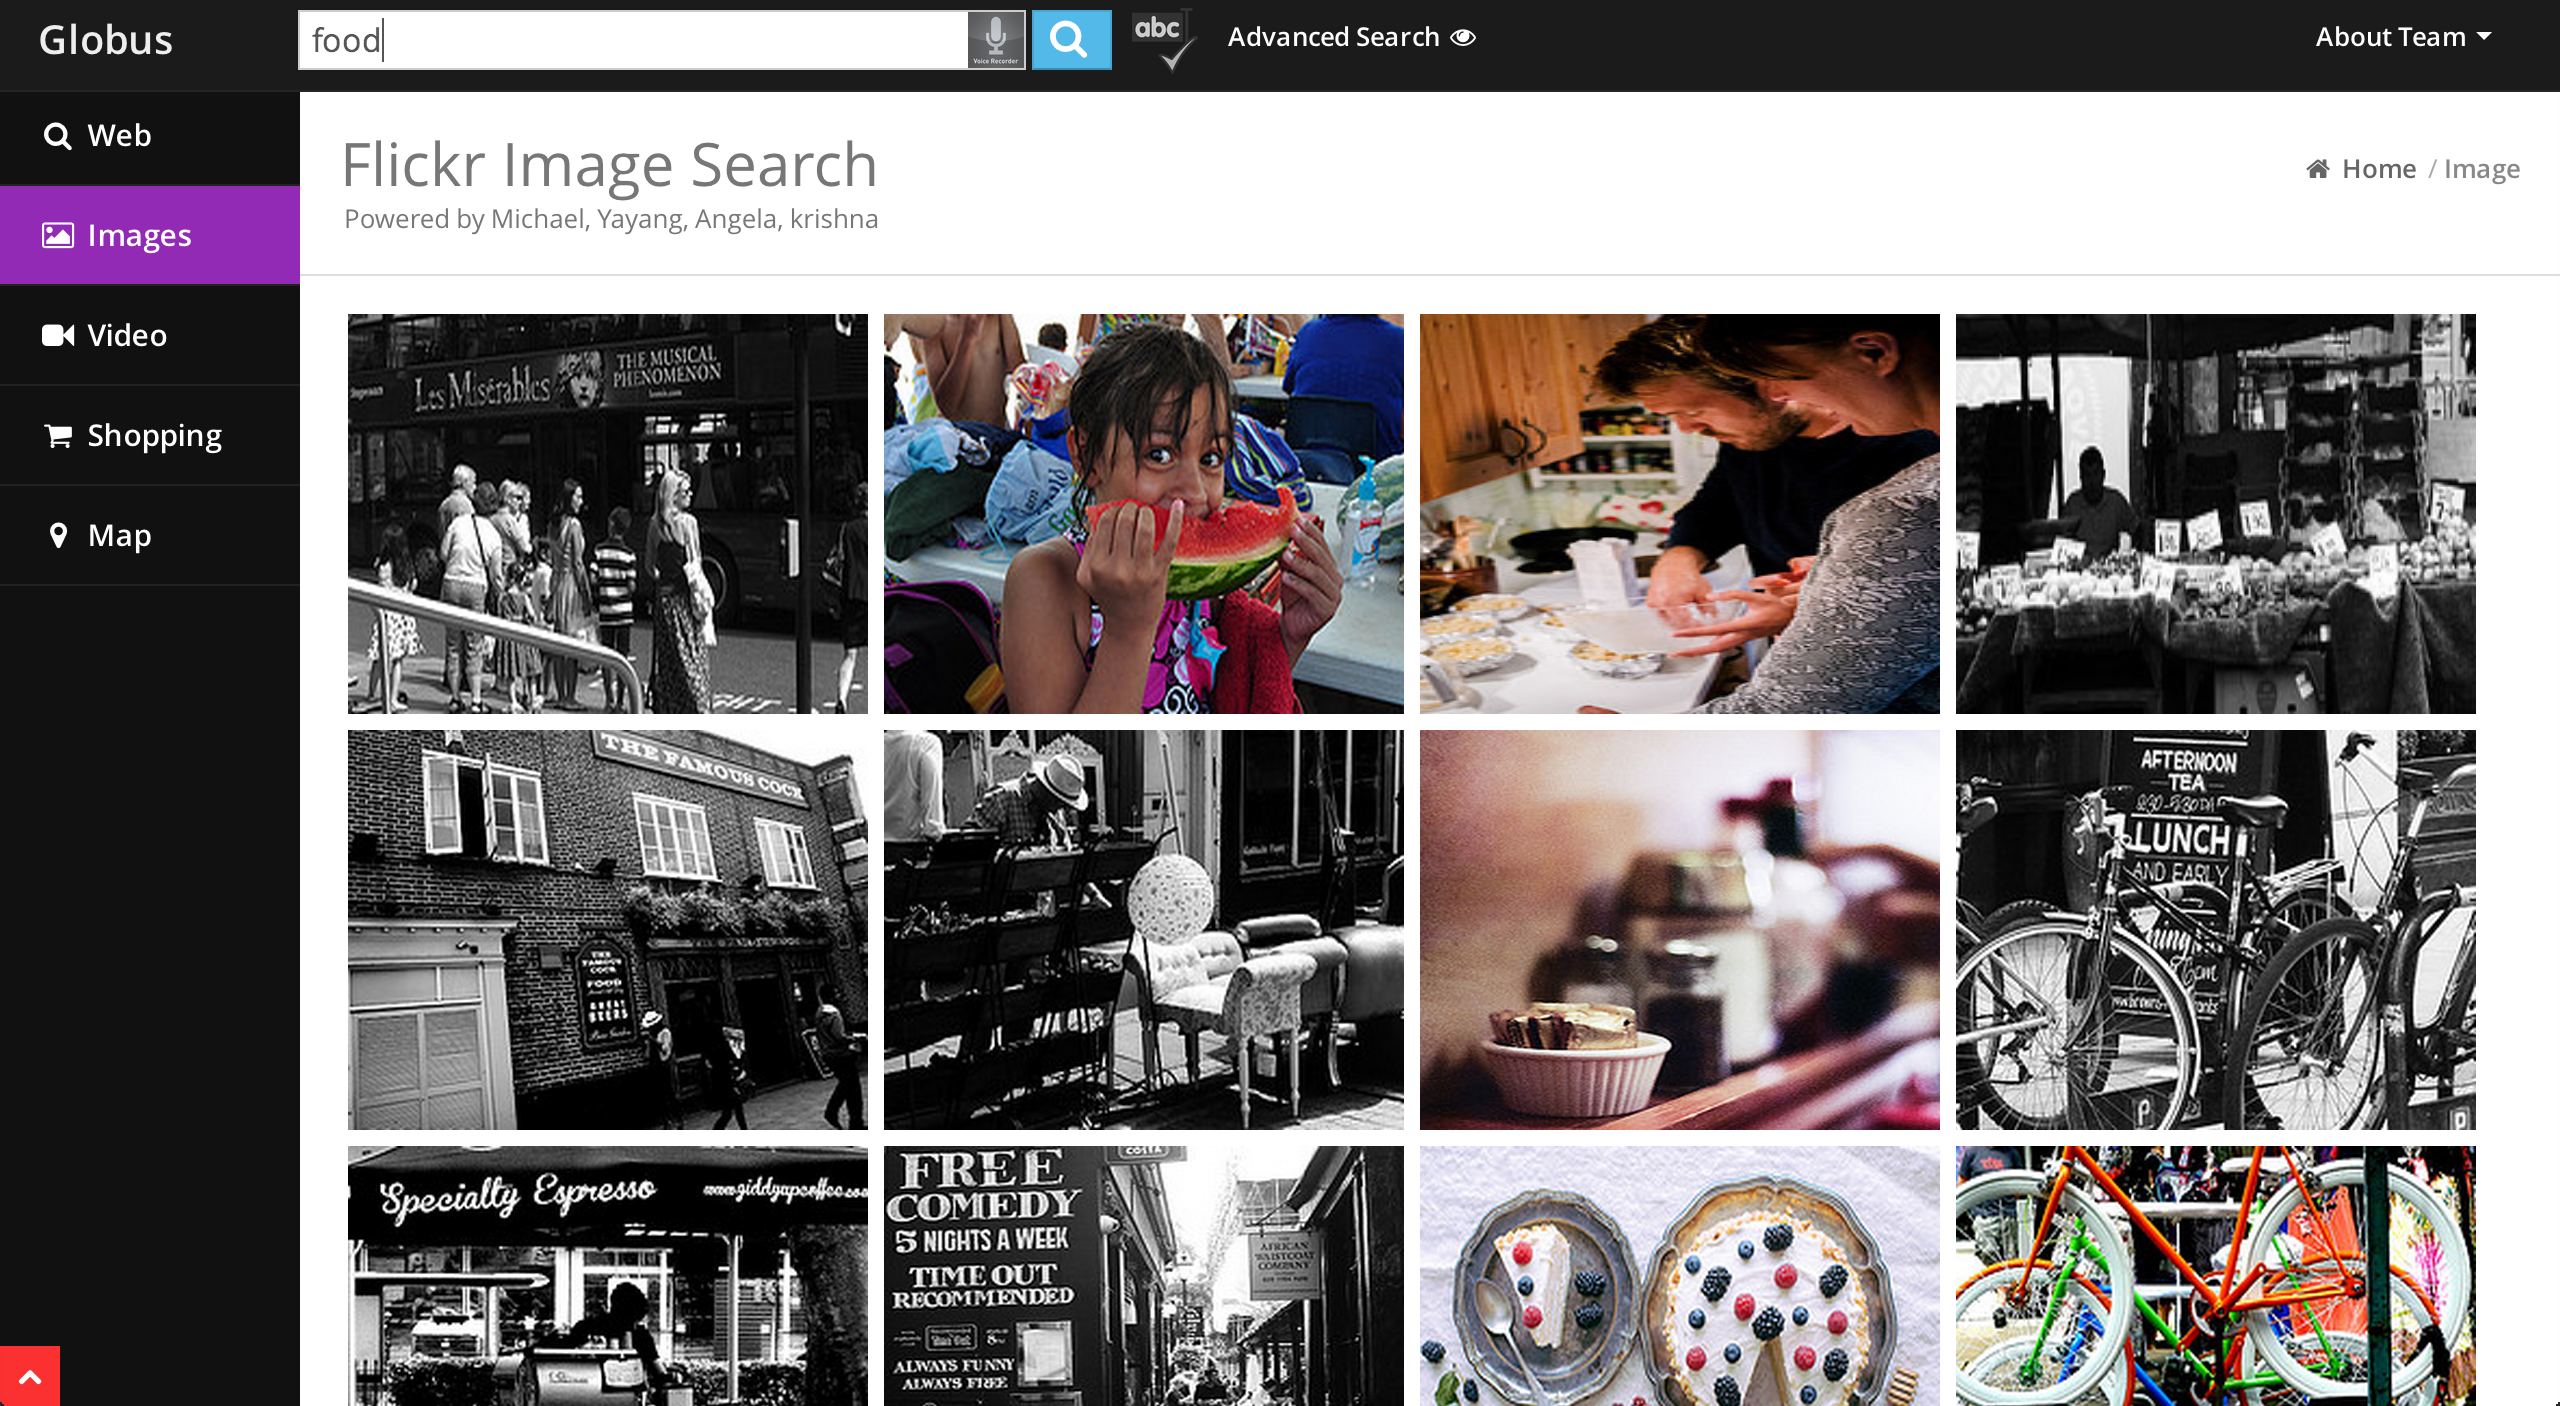
\includegraphics[width=1\linewidth]{pic/search4.png}
\end{figure}
\end{frame}

%------------------------------- Crawler -----------------
\begin{frame}
\frametitle{Crawler}
\begin{figure}
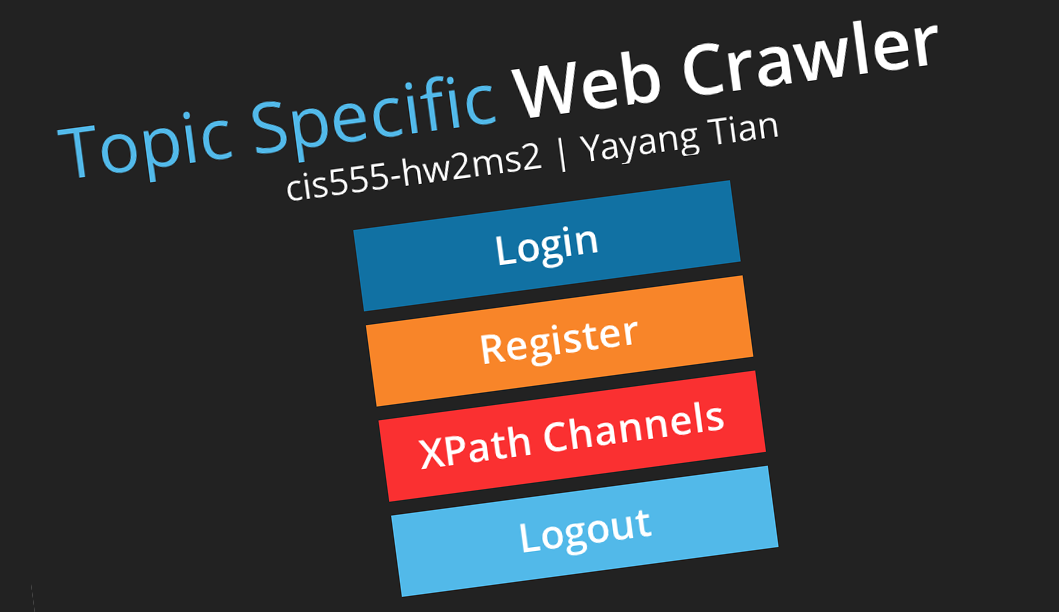
\includegraphics[width=1\linewidth]{pic/crawler1.png}
\end{figure}
\end{frame}
\begin{frame}
\frametitle{Crawler}
\begin{figure}
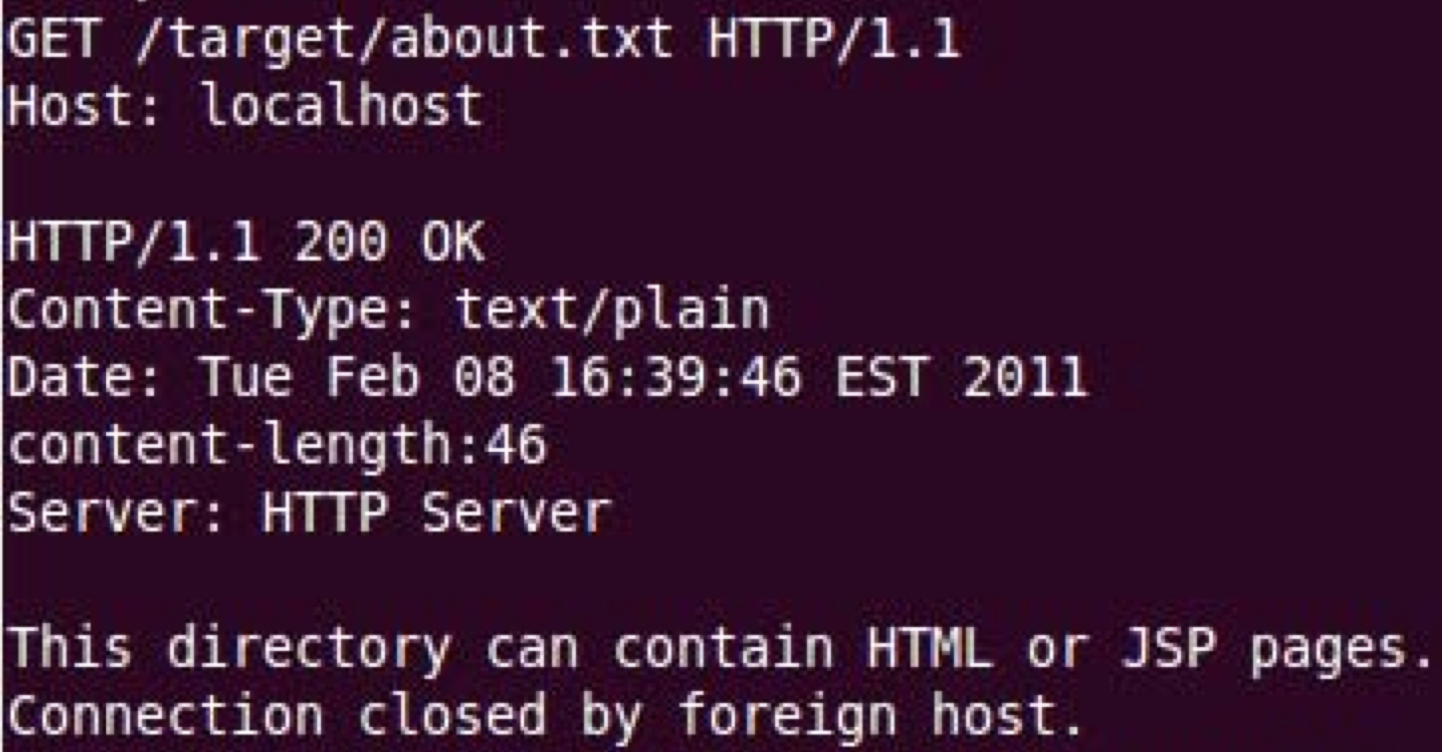
\includegraphics[width=1\linewidth]{pic/crawler2.png}
\end{figure}
\end{frame}
\begin{frame}
\frametitle{Crawler}
\begin{figure}
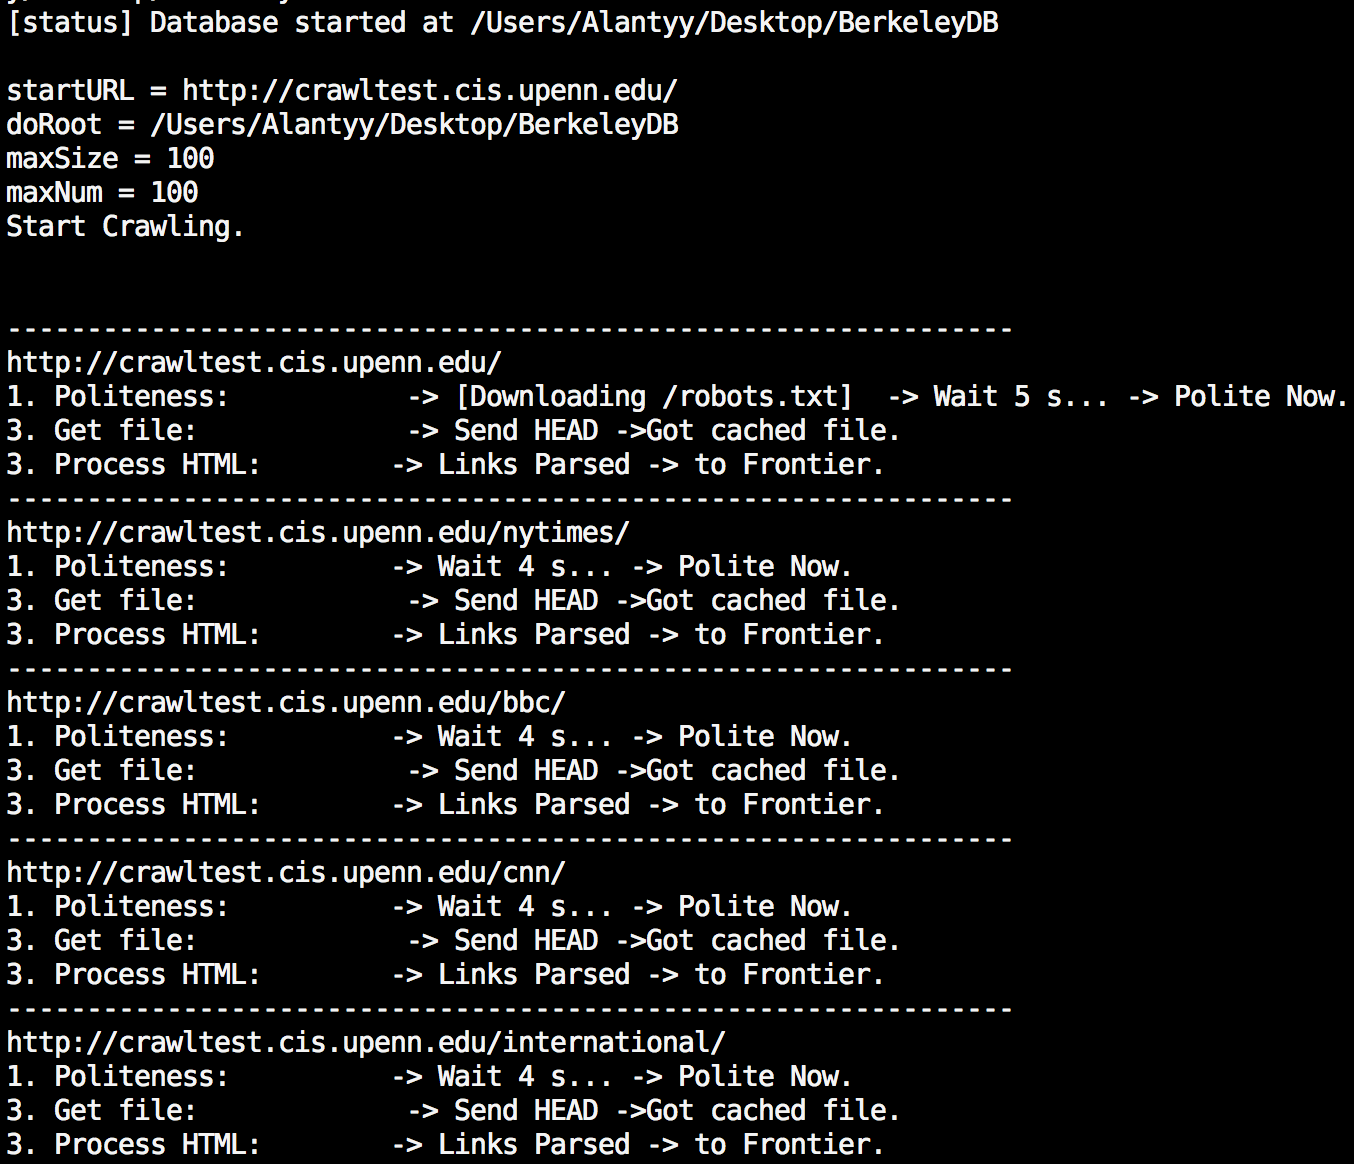
\includegraphics[width=1\linewidth]{pic/crawler3.png}
\end{figure}
\end{frame}


%------------------------------- Distributed Caching -----------------
\begin{frame}
\frametitle{DHTCaching}
\begin{figure}
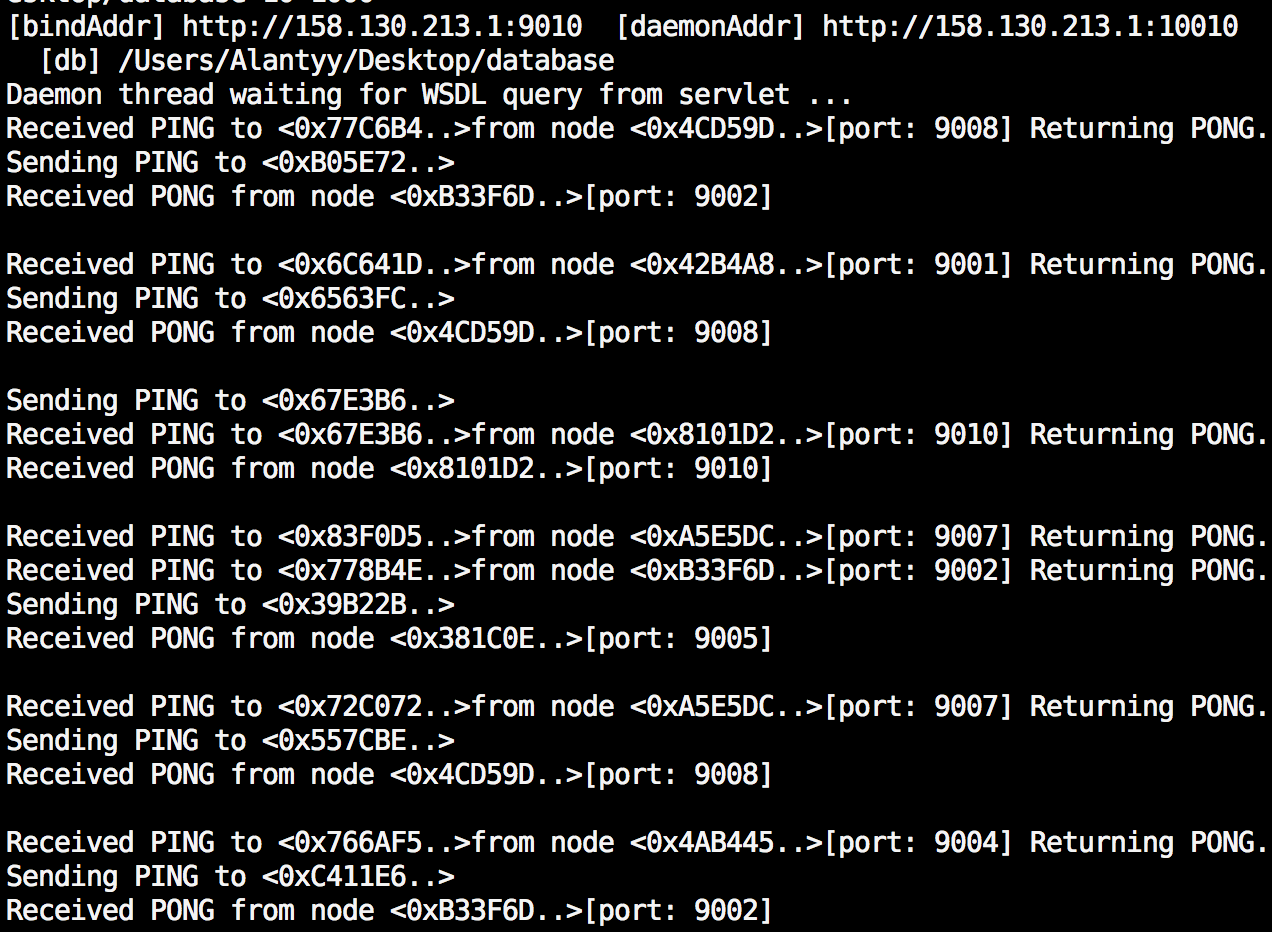
\includegraphics[width=1\linewidth]{pic/caching1.png}
\end{figure}
\end{frame}
\begin{frame}
\frametitle{DHTCaching}
\begin{figure}
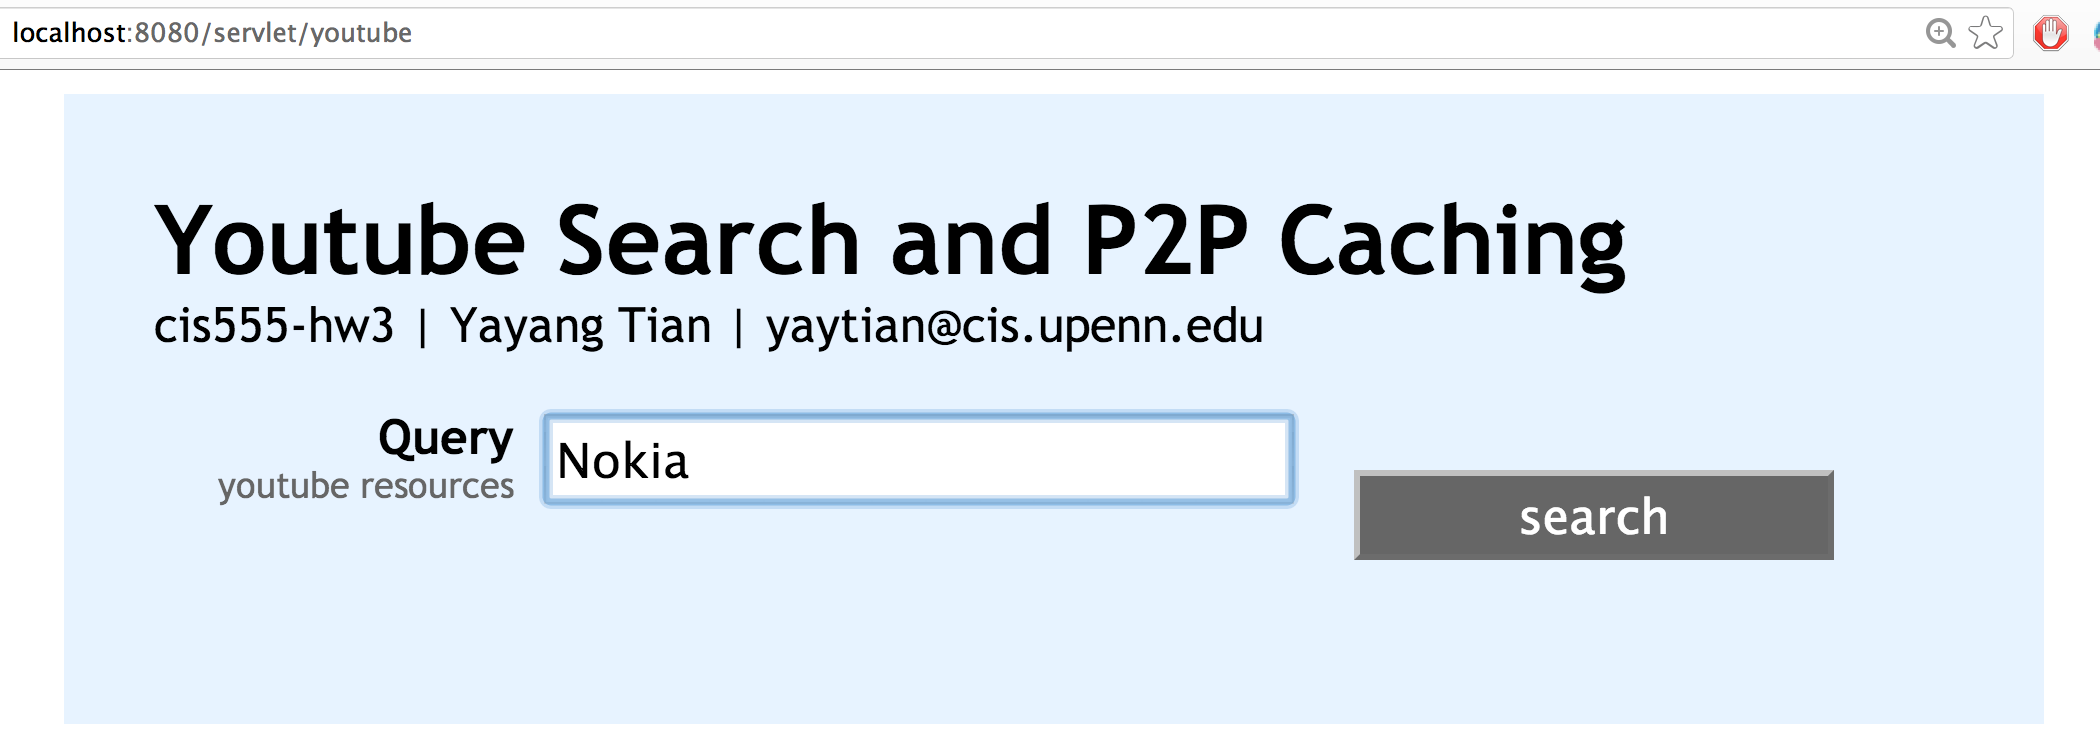
\includegraphics[width=1\linewidth]{pic/caching2.png}
\end{figure}
\end{frame}





%------------------------------- Twitter -----------------
\begin{frame}
\frametitle{TwitterAffect}
\begin{figure}
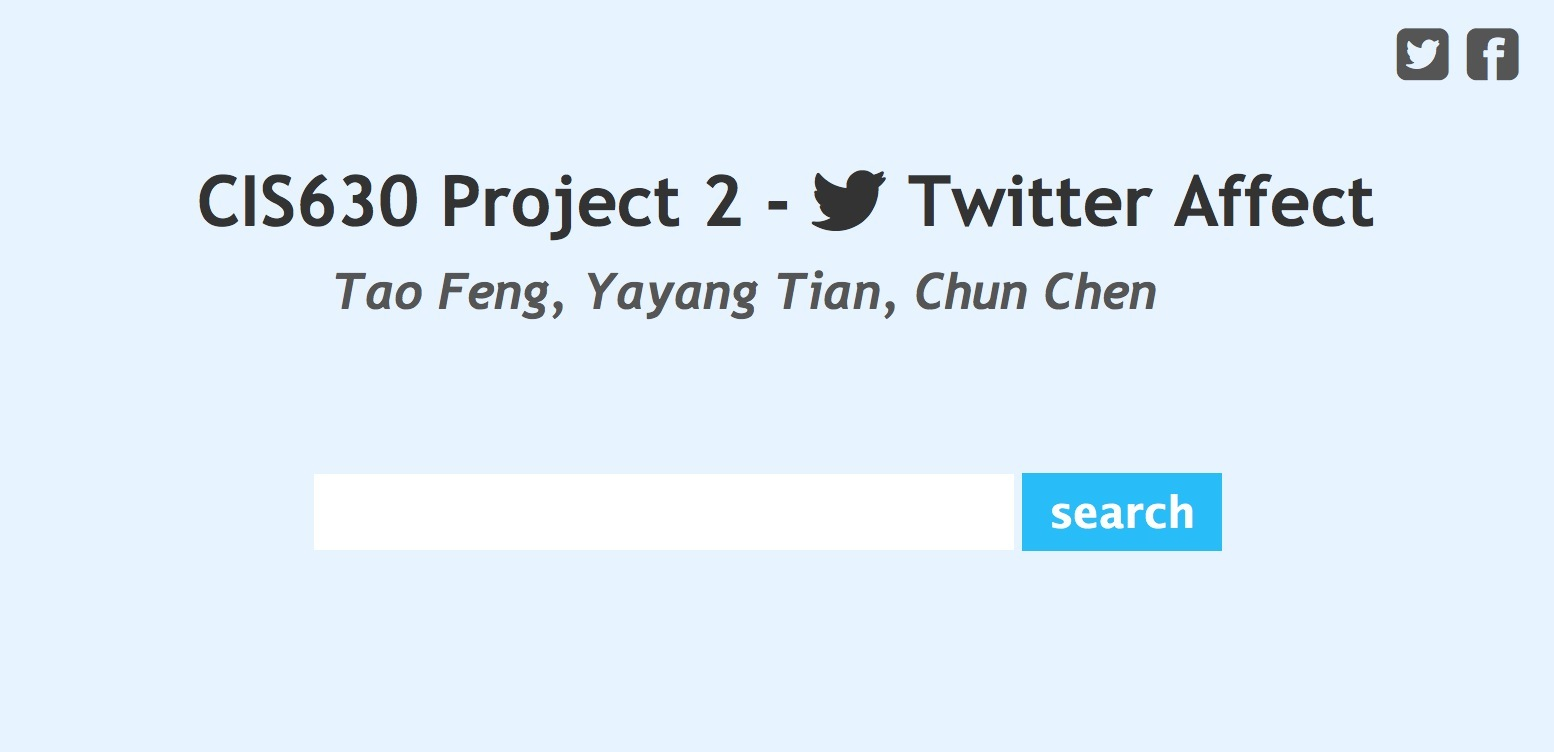
\includegraphics[width=1\linewidth]{pic/twitter1.jpeg}
\end{figure}
\end{frame}
\begin{frame}
\frametitle{TwitterAffect}
\begin{figure}
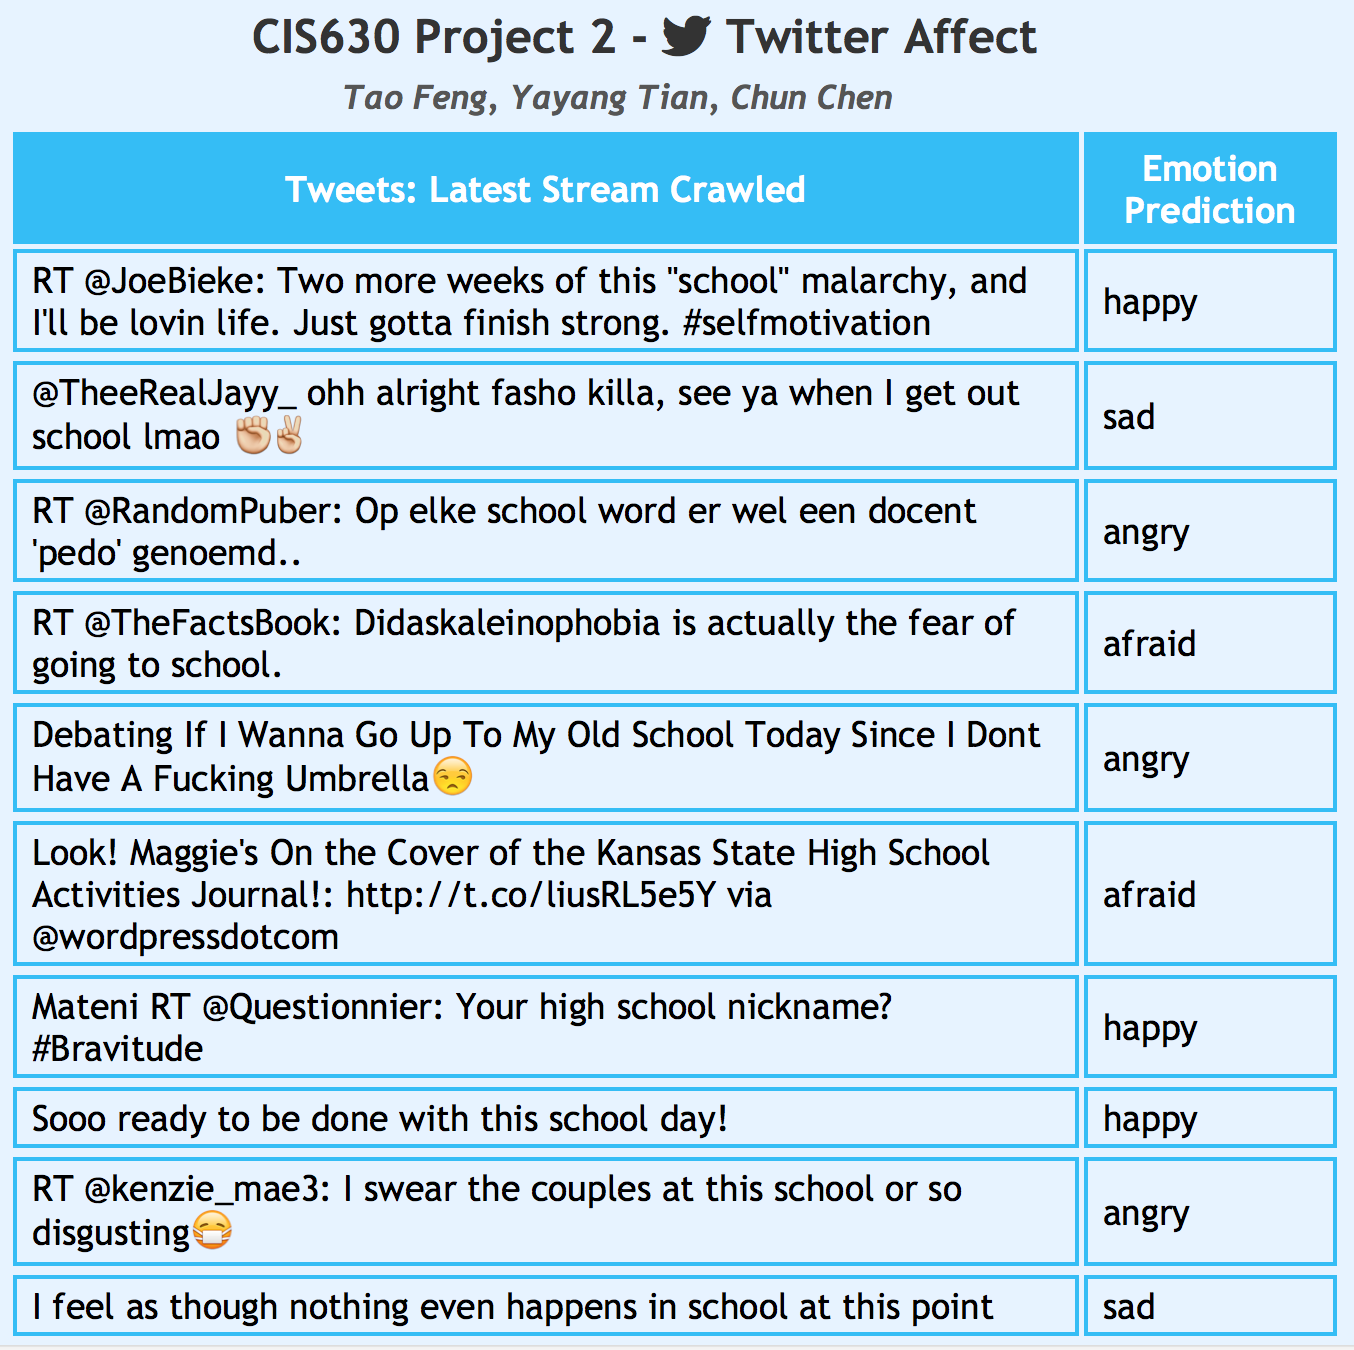
\includegraphics[width=1\linewidth]{pic/twitter2.png}
\end{figure}
\end{frame}

%------------------------------- NLP -----------------
\begin{frame}
\frametitle{NLP-Crowdsourcing}
\begin{figure}
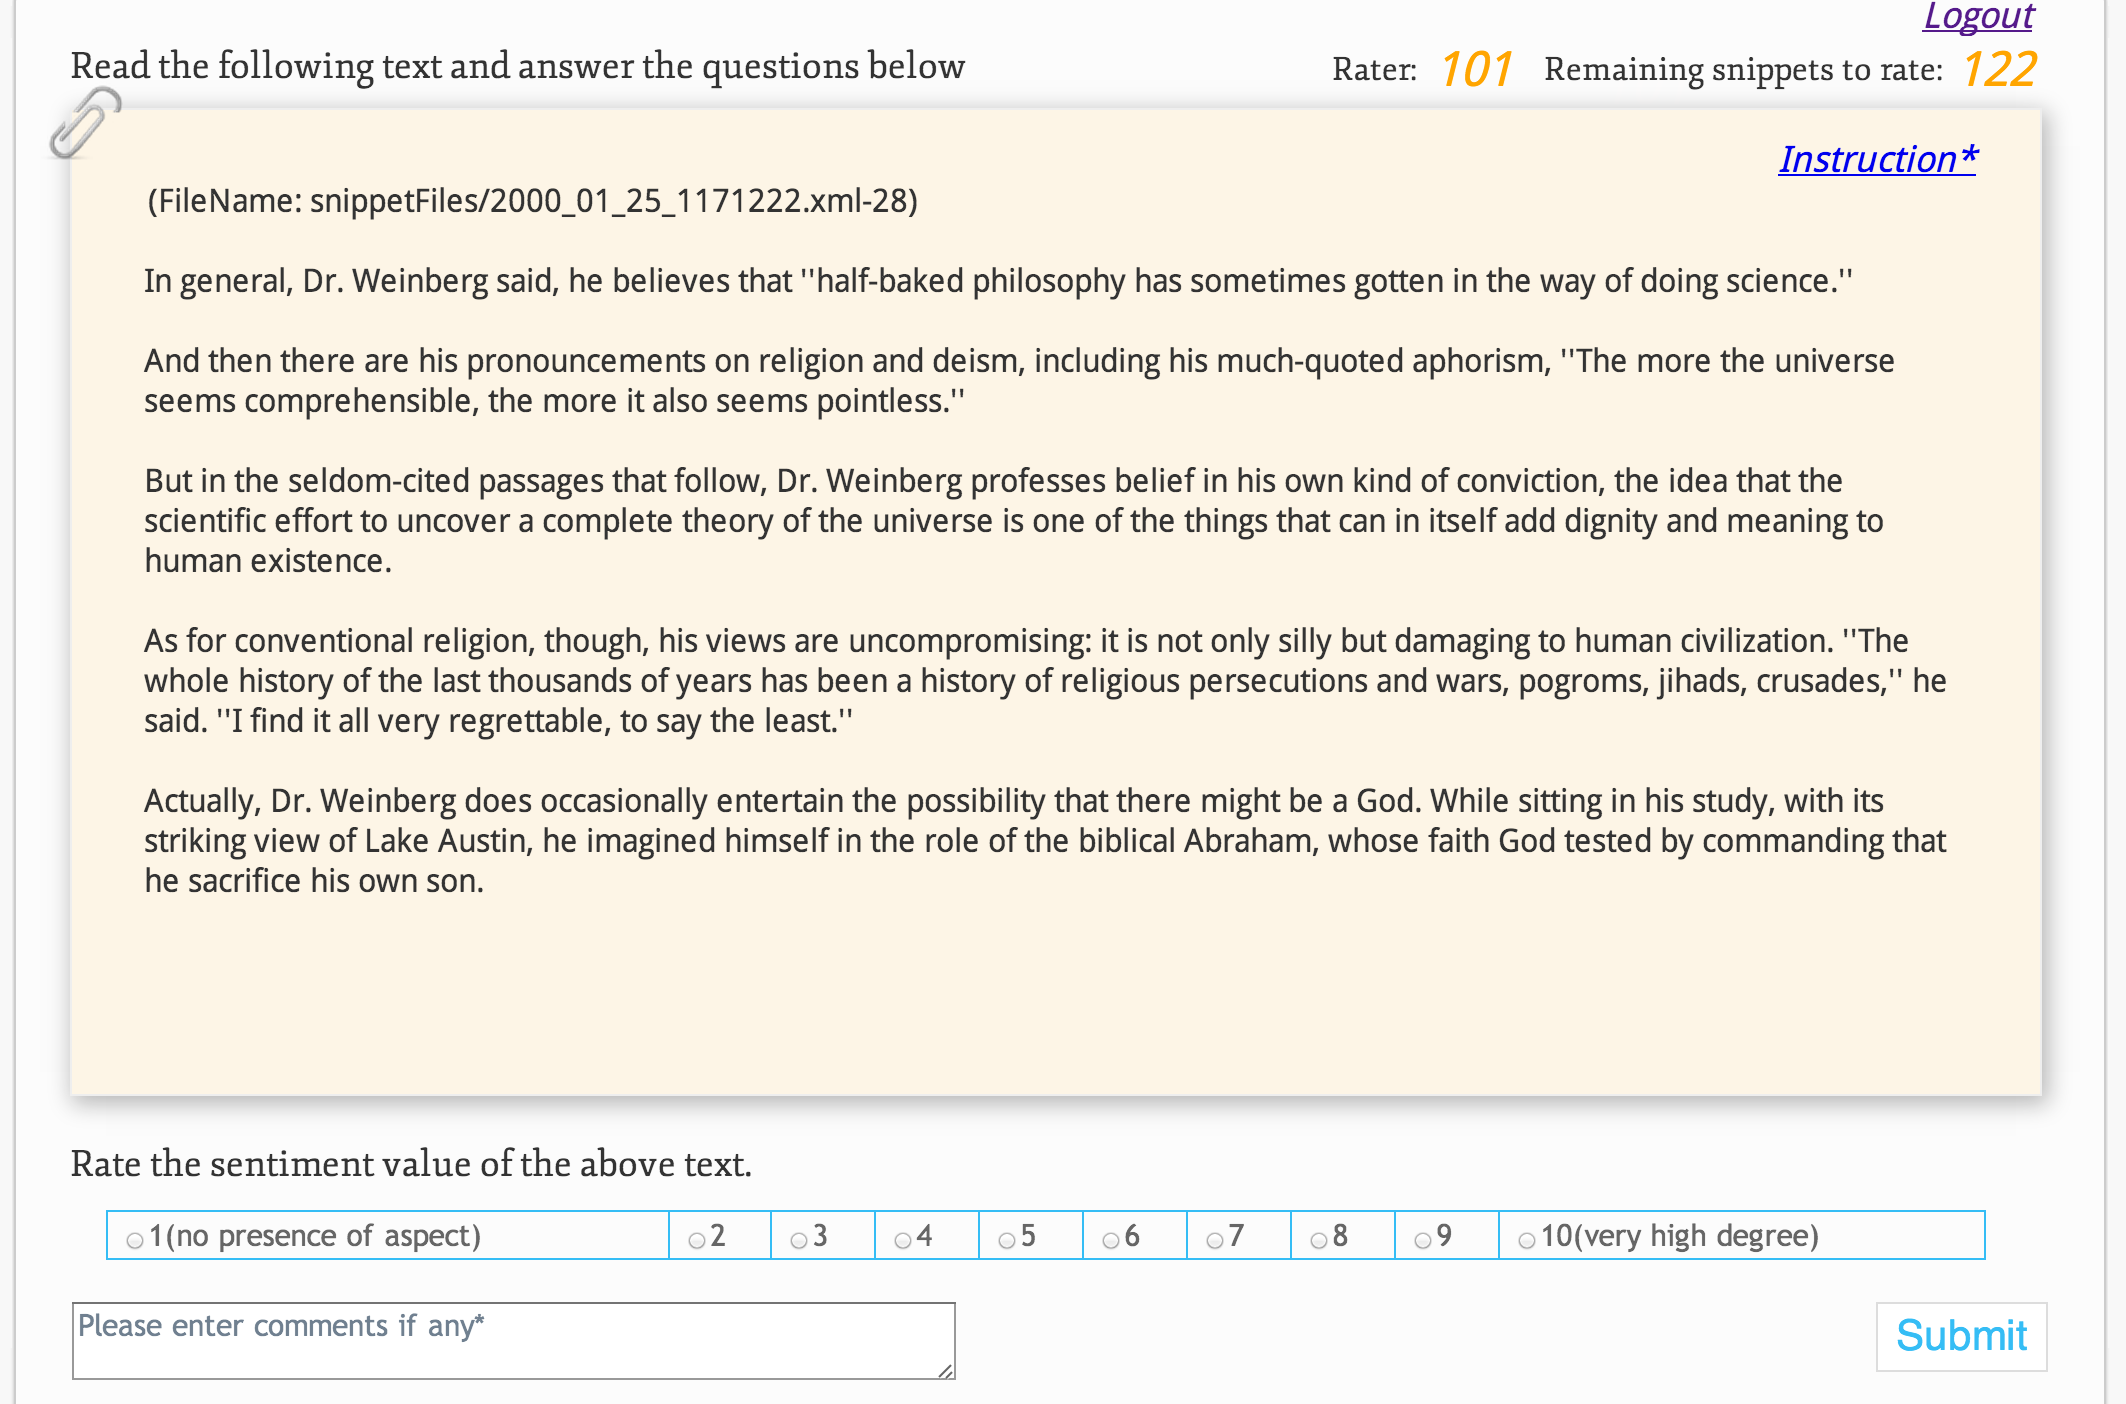
\includegraphics[width=1\linewidth]{pic/annotation1.png}
\end{figure}
\end{frame}
\begin{frame}
\frametitle{NLP-Crowdsourcing}
\begin{figure}
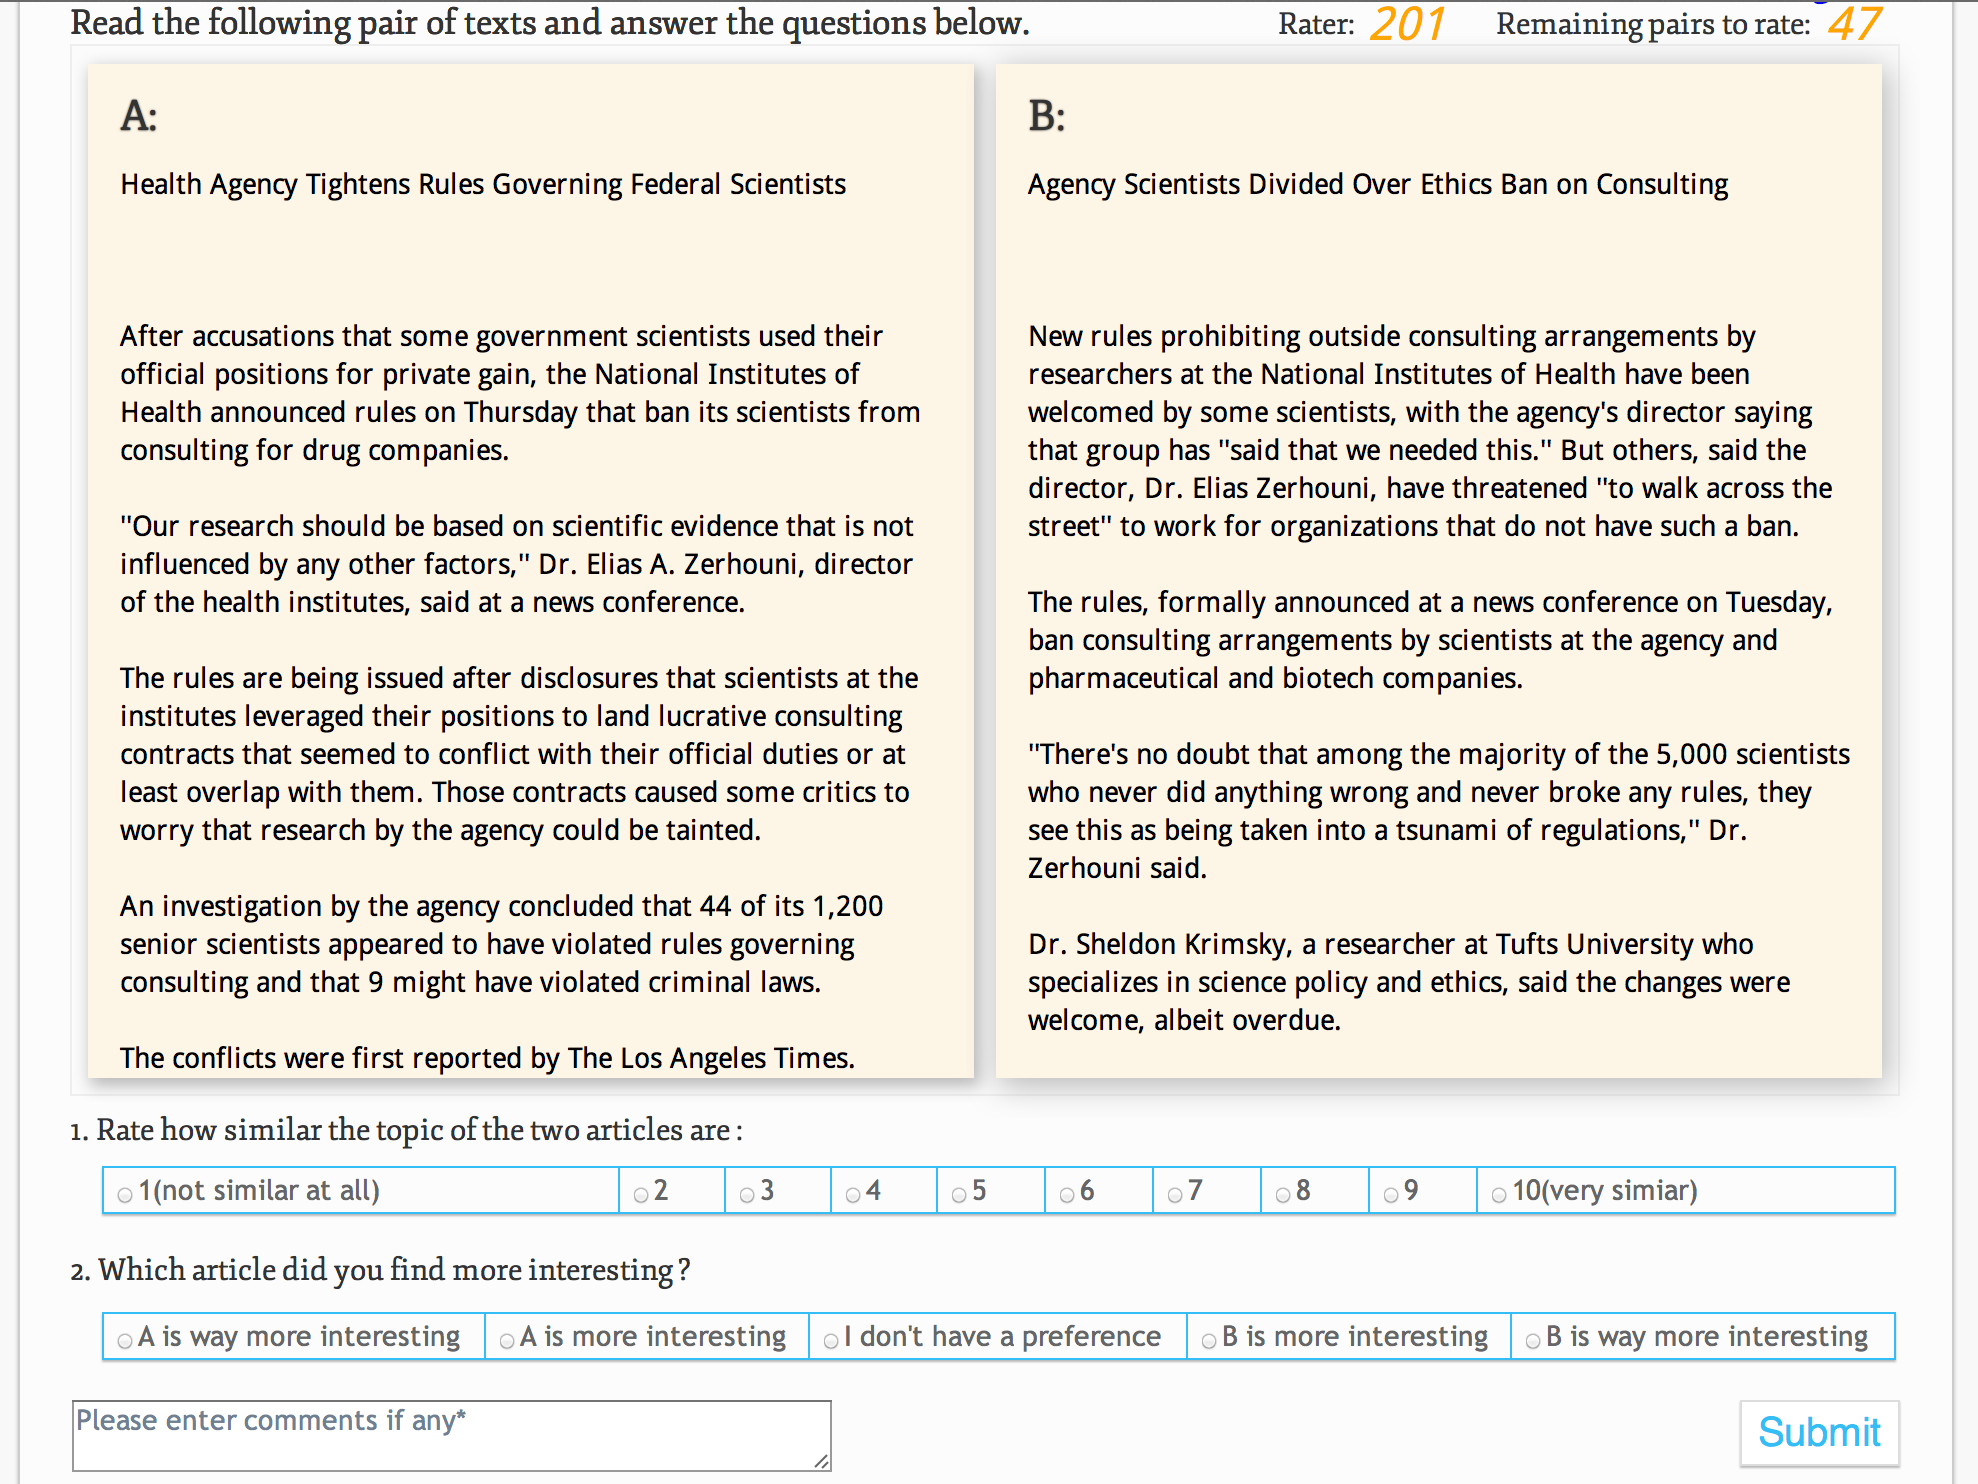
\includegraphics[width=1\linewidth]{pic/annotation2.png}
\end{figure}
\end{frame}
\begin{frame}
\frametitle{NLP-Crowdsourcing}
\begin{figure}
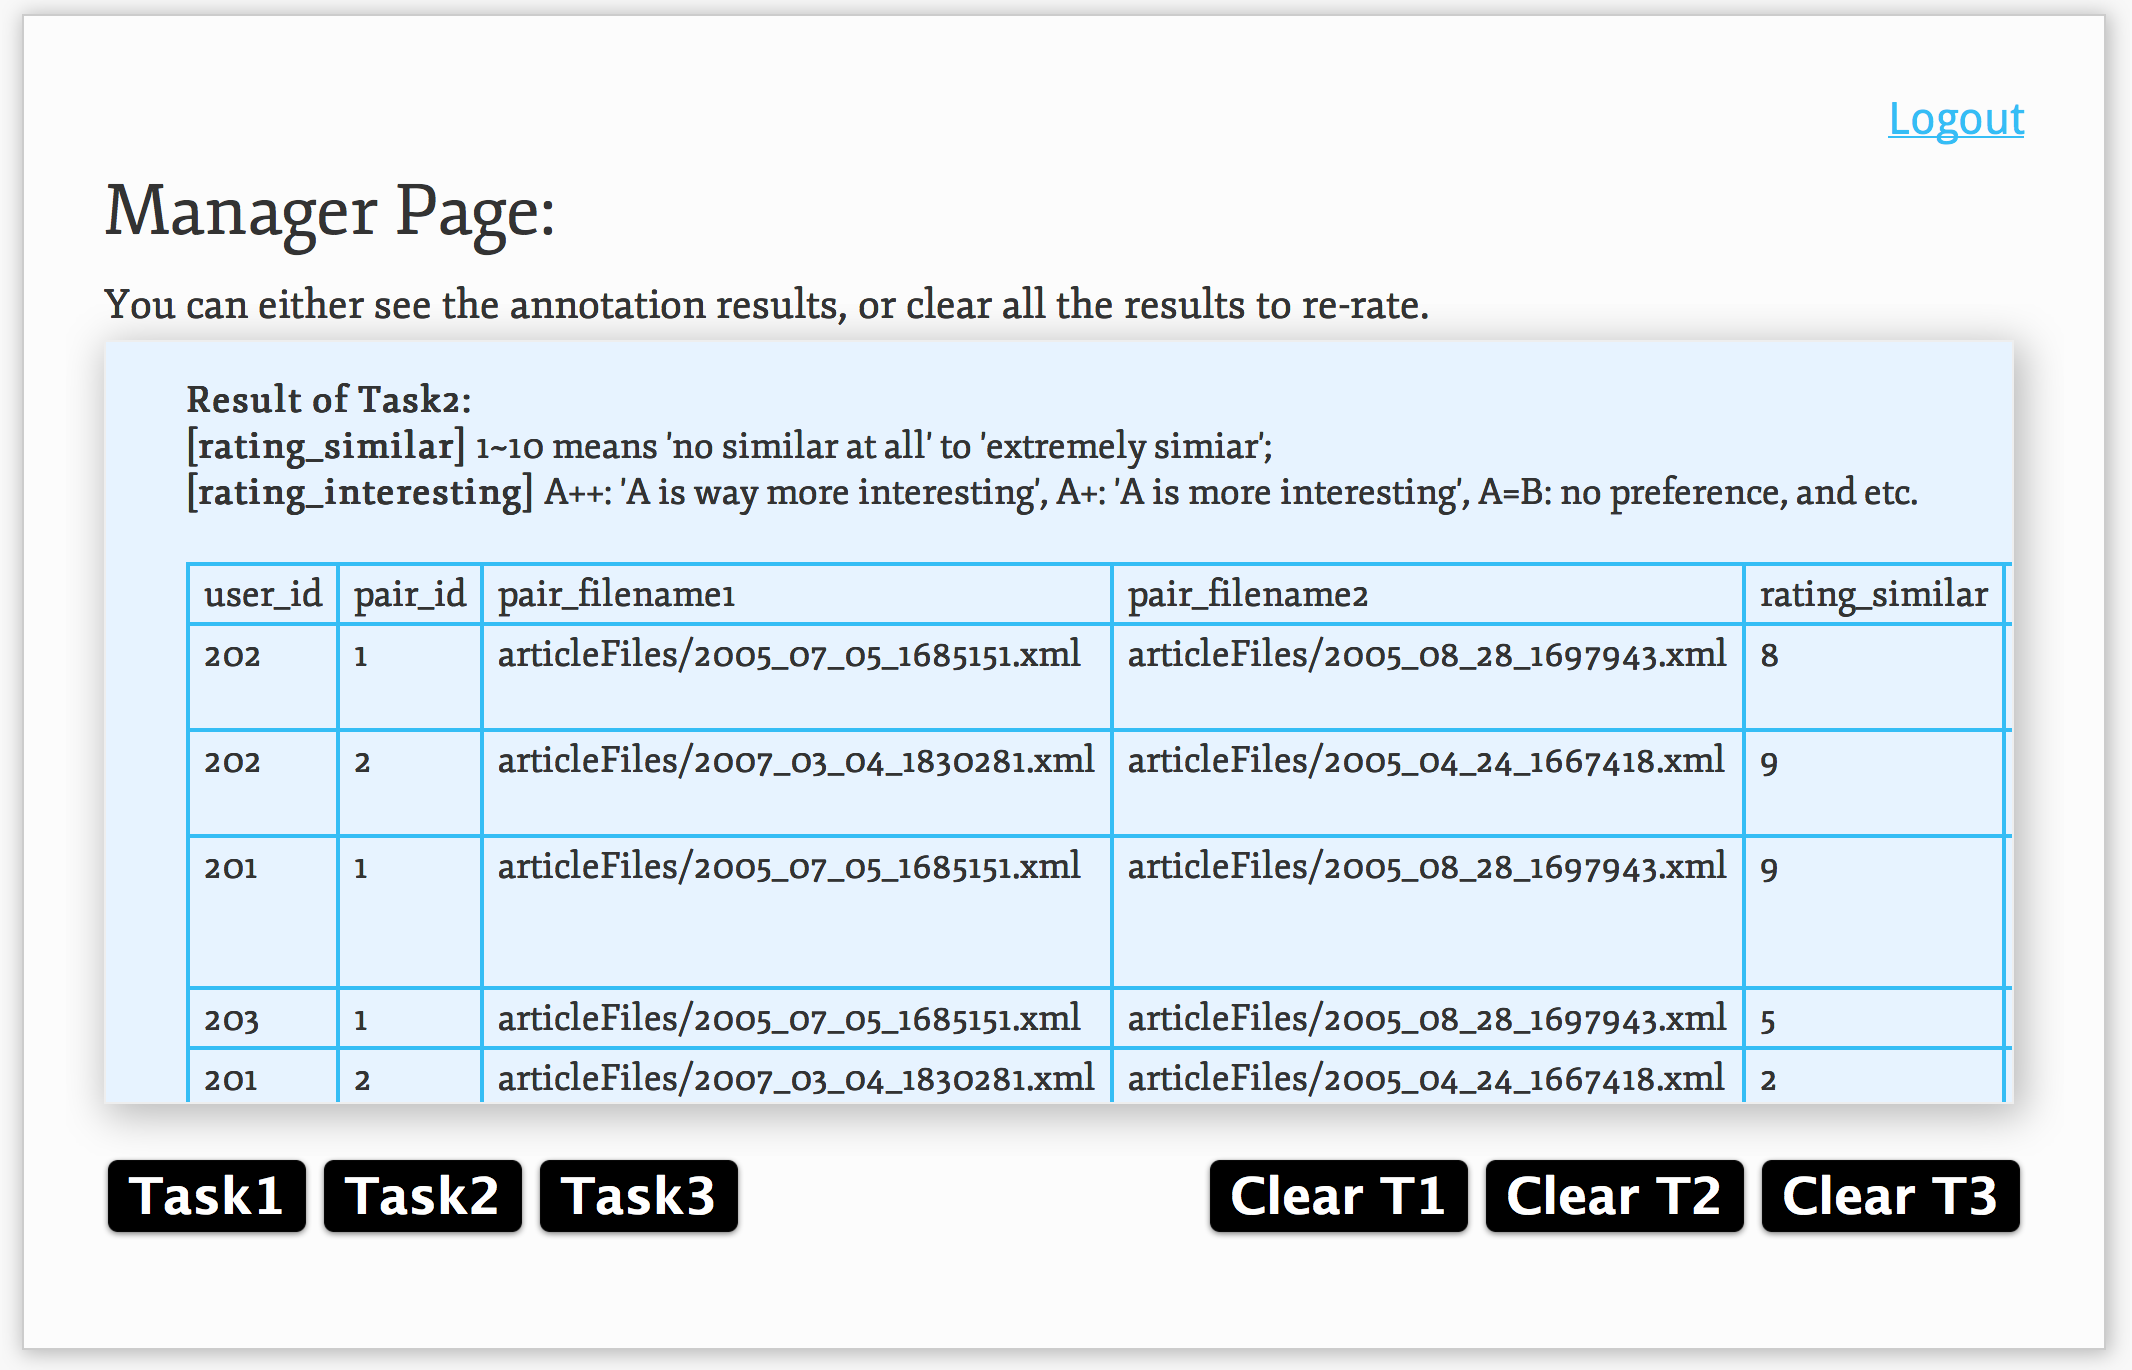
\includegraphics[width=1\linewidth]{pic/annotation3.png}
\end{figure}
\end{frame}


%------------------------------- summary -----------------
\begin{frame}
\frametitle{Summarization}
\begin{figure}
\includegraphics[width=0.75\linewidth]{pic/summary.png}
\end{figure}
\end{frame}


%------------------------------- database -----------------
\begin{frame}
\frametitle{MonopolyOlympics}
\begin{figure}
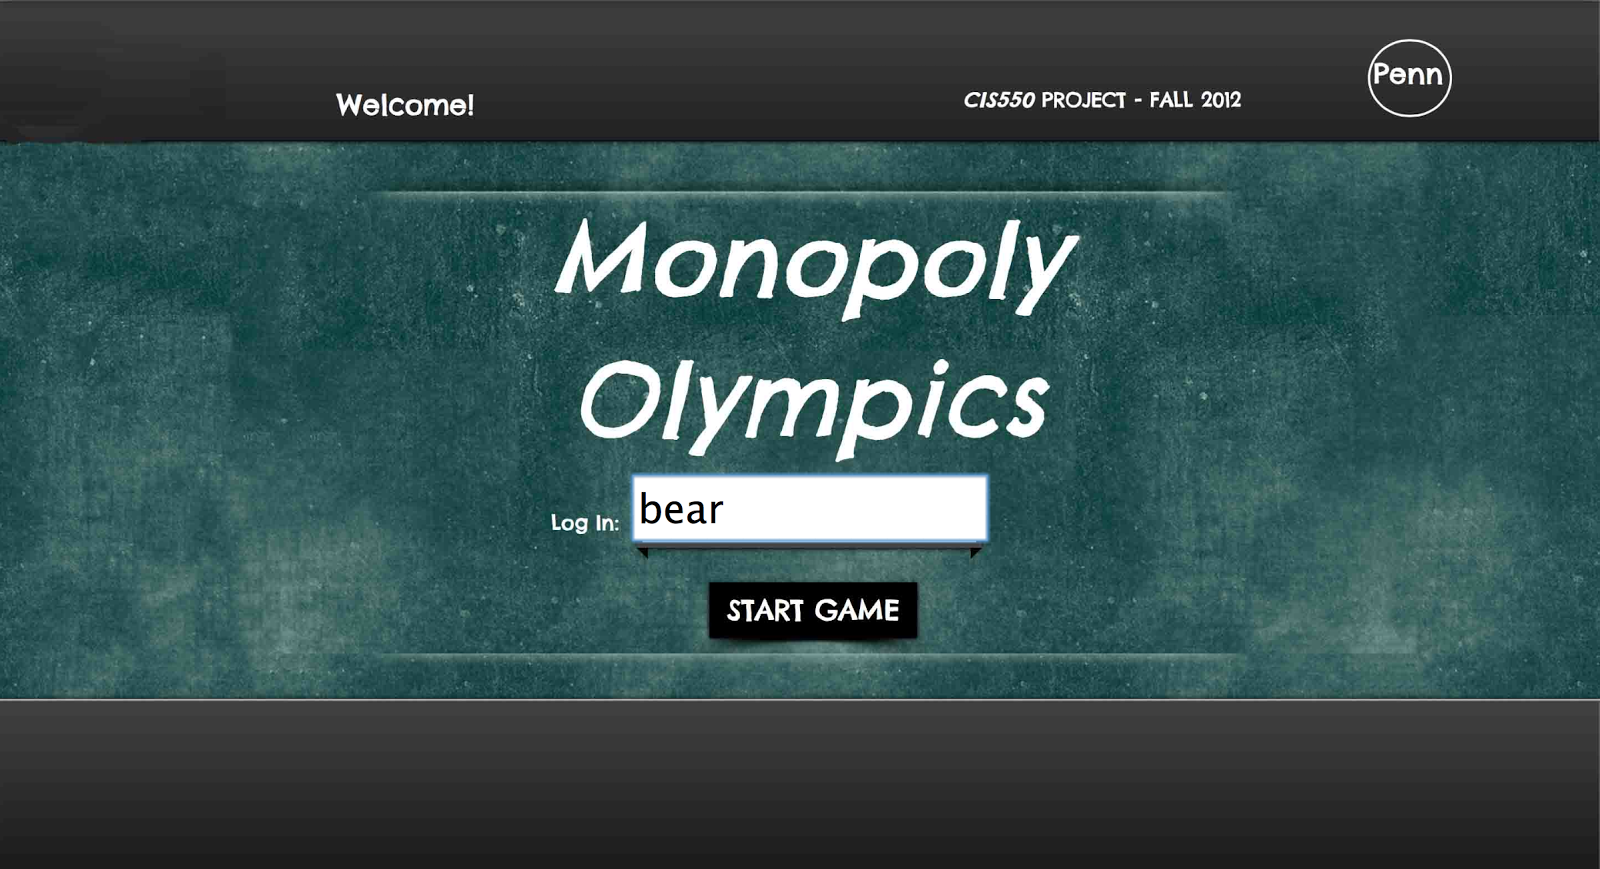
\includegraphics[width=1\linewidth]{pic/database1.png}
\end{figure}
\end{frame}
\begin{frame}
\frametitle{MonopolyOlympics}
\begin{figure}
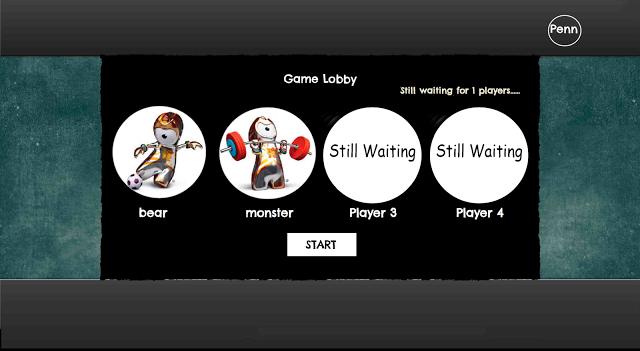
\includegraphics[width=1\linewidth]{pic/database2.png}
\end{figure}
\end{frame}
\begin{frame}
\frametitle{MonopolyOlympics}
\begin{figure}
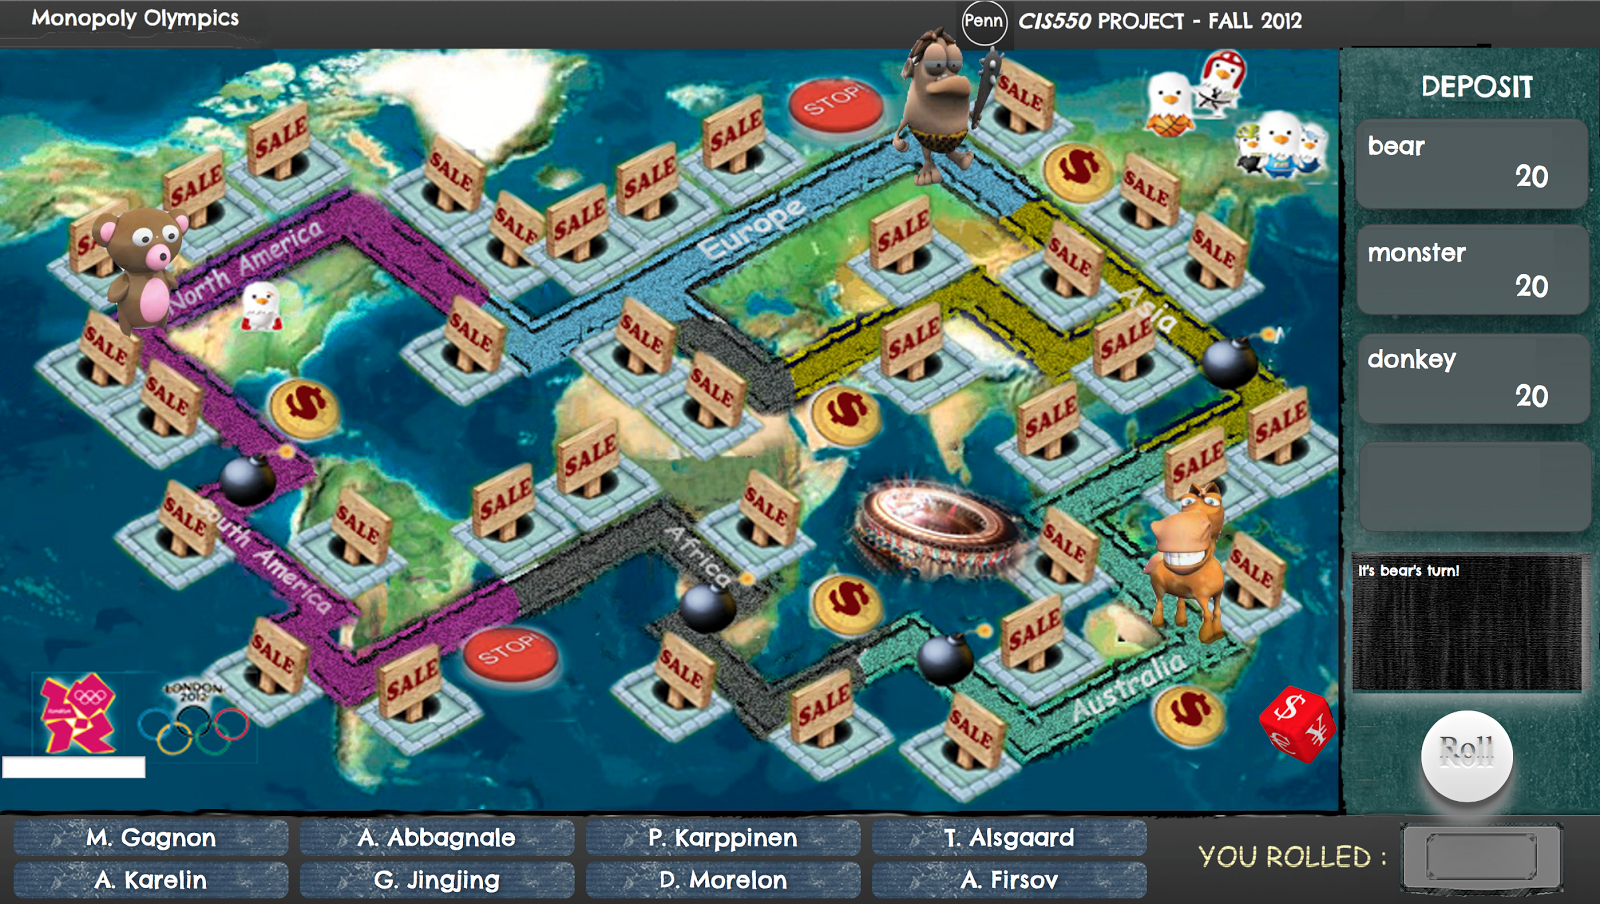
\includegraphics[width=1\linewidth]{pic/database3.png}
\end{figure}
\end{frame}



%------------------------------- Android -----------------
\begin{frame}
\frametitle{Mobile - FancyCooler}
\begin{figure}
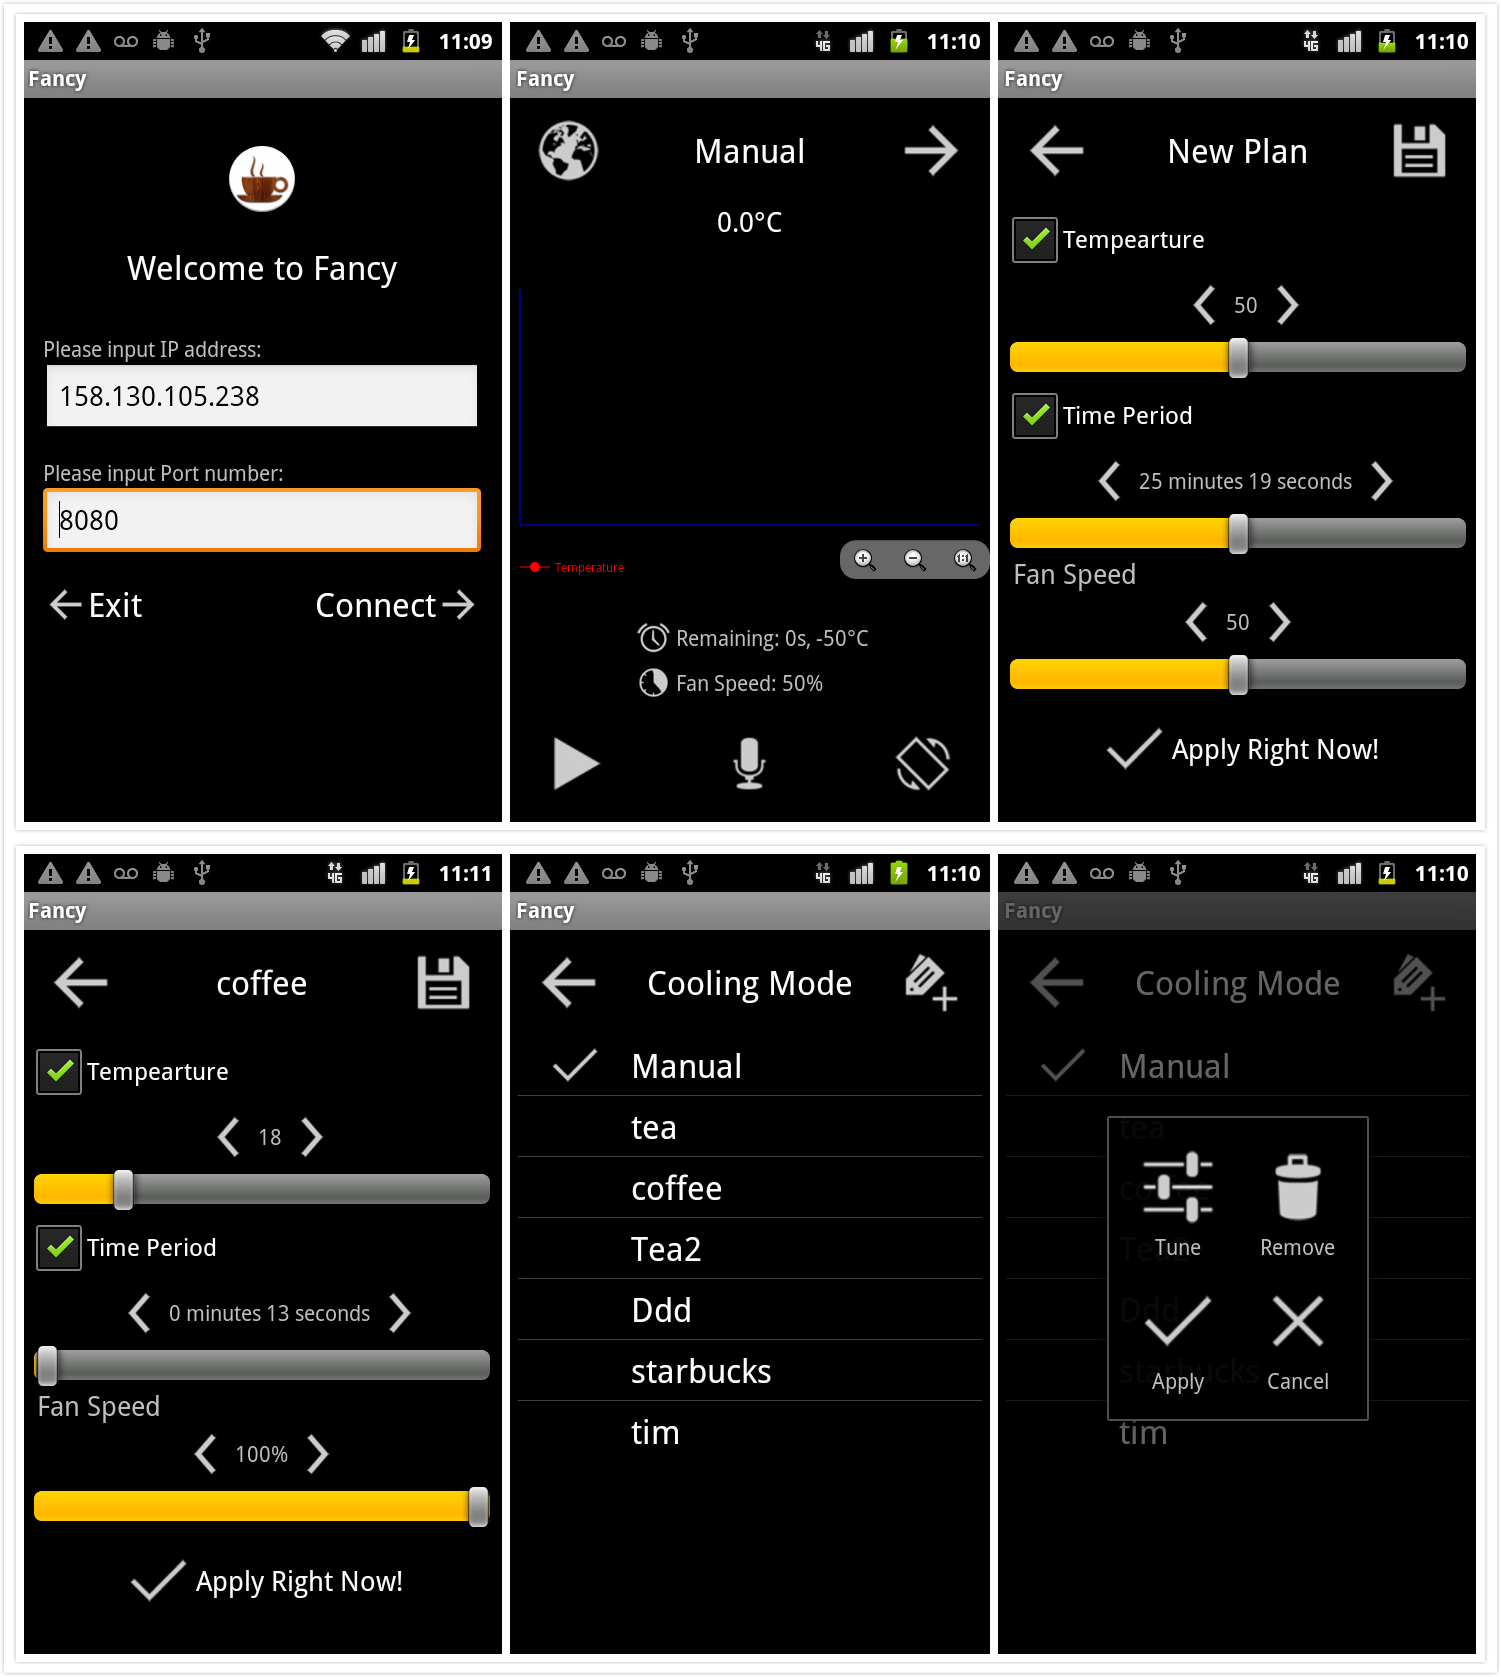
\includegraphics[width=0.65\linewidth]{pic/mobile1.png}
\end{figure}
\end{frame}
\begin{frame}
\frametitle{Mobile}
\begin{figure}
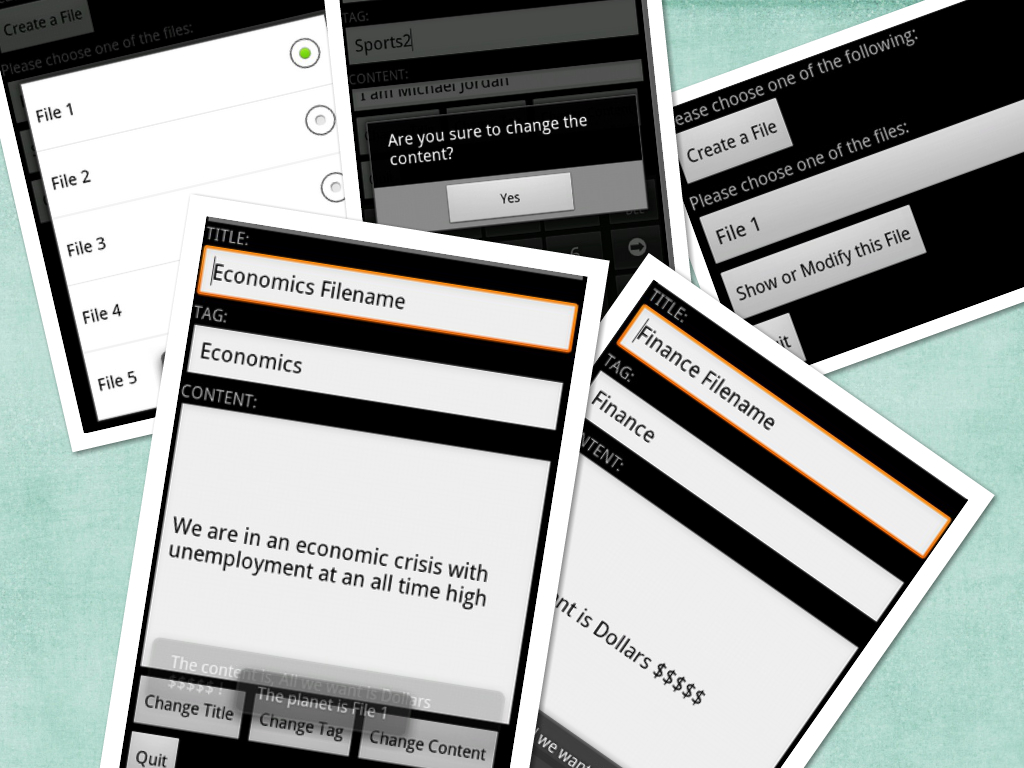
\includegraphics[width=1\linewidth]{pic/mobile2.jpg}
\end{figure}
\end{frame}
\begin{frame}
\frametitle{Mobile}
\begin{figure}
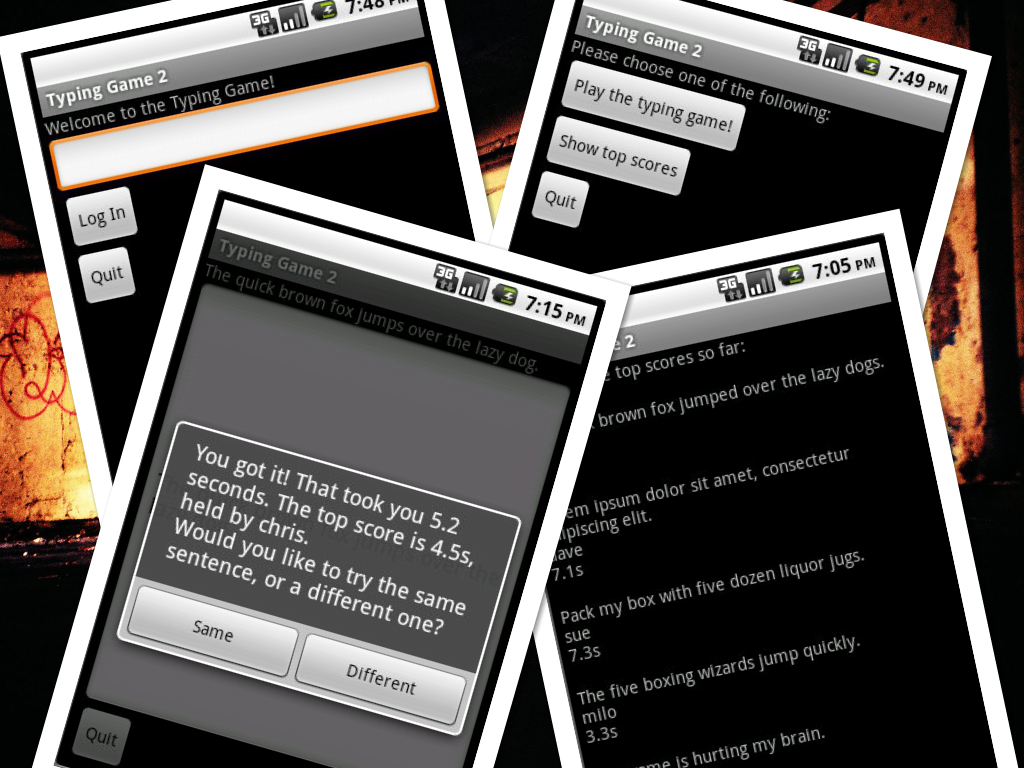
\includegraphics[width=1\linewidth]{pic/mobile3.jpg}
\end{figure}
\end{frame}





\begin{frame}

\frametitle{Projects Summary}

\textbf{Distributed Systems}
\begin{itemize}
\item Distributed Web Search Engine: MiniGoogle
\item DHT-based Search Engine: PennSearch 
\item Distributed Caching and Web Services
\item Web Crawler with Multithreaded Server 
\end{itemize}


\textbf{Data Mining}
\begin{itemize}
\item Amazon Reviews Data Mining
\item Tweets Emotion Prediction
\item New York Times Summarization
\item Wall Street Journal Crowdsouring Website
\end{itemize}

\textbf{Others}
\begin{itemize}
\item Mobile Applications
\item Database Website on GAE
\end{itemize}

\end{frame}

%------------------------------------------------

\begin{frame}
\Huge{\centerline{The End}}
\end{frame}

%----------------------------------------------------------------------------------------

\end{document} 